\documentclass[10pt]{article}

\usepackage[T1]{fontenc}
\usepackage[utf8]{inputenc}
\usepackage{lmodern}
\usepackage{microtype}
\usepackage[margin=0.72in,columnsep=0.24in]{geometry}
\usepackage{amsmath,amssymb,bm}
\usepackage{booktabs}
\usepackage{graphicx}
\usepackage{float}
\usepackage{multirow}
\usepackage{caption}
\usepackage{subcaption}
\usepackage{enumitem}
\usepackage{xspace}
\usepackage{cuted}
\usepackage{xcolor}
\usepackage{xurl}
\usepackage[numbers,sort&compress]{natbib}
\usepackage[
  colorlinks=true,
  linkcolor=blue!55!black,
  citecolor=blue!55!black,
  urlcolor=blue!55!black
]{hyperref}
\usepackage[capitalise,noabbrev]{cleveref}

\setlist{nosep,leftmargin=*}
\setlength{\textfloatsep}{8pt plus 2pt minus 2pt}
\setlength{\floatsep}{8pt plus 2pt minus 2pt}
\setlength{\intextsep}{8pt plus 2pt minus 2pt}
\captionsetup{font=small,labelfont=bf}

\newcommand{\method}{LARP-Scaler\xspace}
\newcommand{\R}{\mathbb{R}}
\makeatletter
\newcommand{\LarpFrontMatter}{%
  \begin{@twocolumnfalse}
    \maketitle
    \begin{center}
      \begin{minipage}{0.90\textwidth}
        \centering
        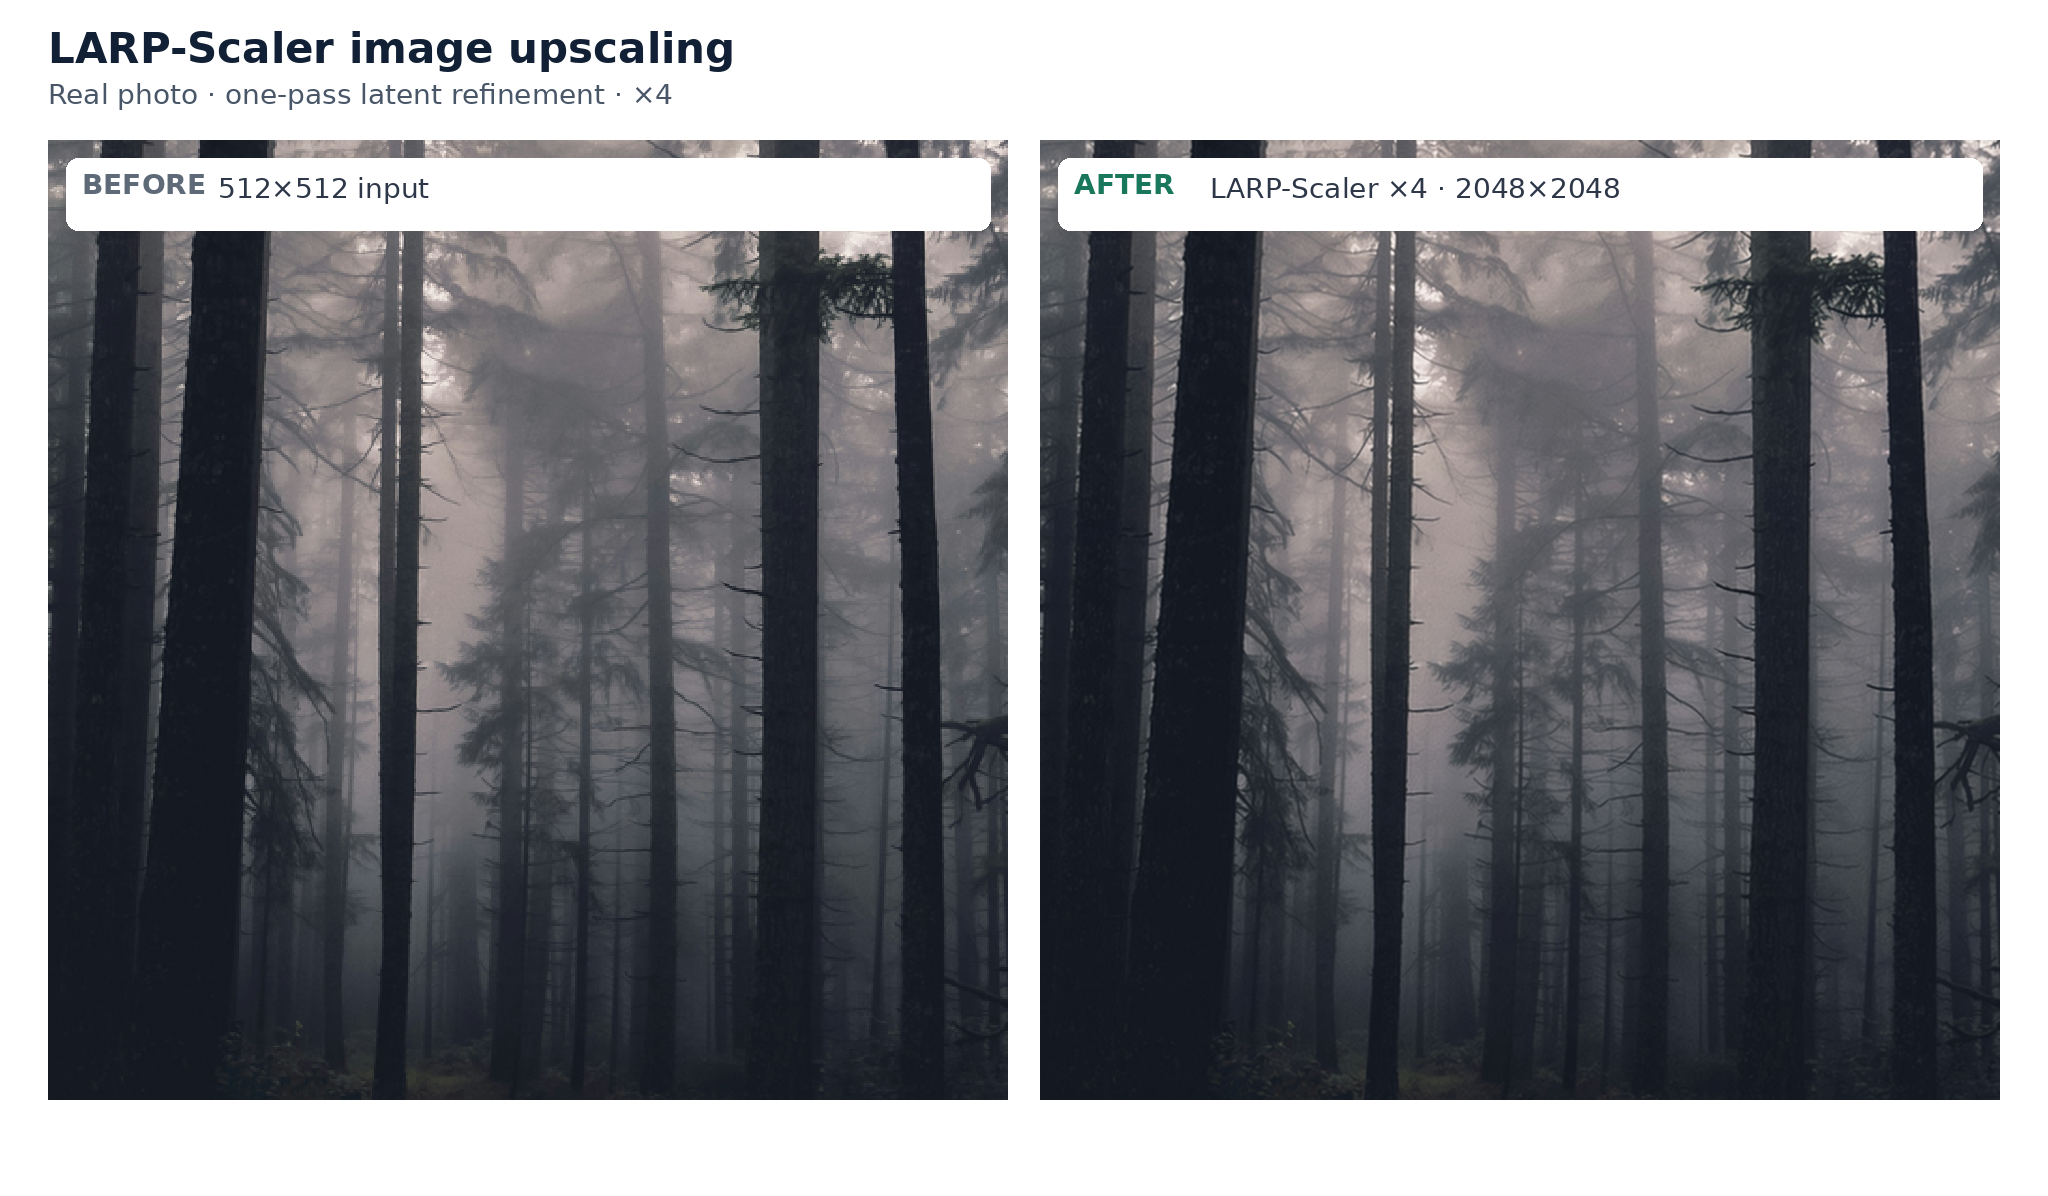
\includegraphics[width=\linewidth]{figures/larp_before_after_hero.png}
      \end{minipage}
    \end{center}
  \end{@twocolumnfalse}%
}
\makeatother

\title{\textbf{LARP-Scaler: Direct Latent Refinement for\\Fast Multi-Scale Image Super-Resolution}}

\author{
  Vladimir Melnikov \quad Maxim Manushin \quad Ilia Kuleshov\\[2pt]
  \small \url{https://github.com/Vovanm88/LARP-Scaler}
}

\date{Draft preprint, July 2026}
\hypersetup{
  pdftitle={LARP-Scaler: Direct Latent Refinement for Fast Multi-Scale Image Super-Resolution},
  pdfauthor={Vladimir Melnikov, Maxim Manushin, Ilia Kuleshov},
  pdfsubject={Technical preprint on latent image super-resolution}
}

\begin{document}
% The optional argument creates a non-floating full-width banner at the top of
% the first two-column page.  The abstract then fills the remaining space.
\twocolumn[\LarpFrontMatter]

\begin{abstract}
Latent image generators provide expressive priors, but practical
super-resolution must balance synthesized detail against exact reconstruction
and runtime cost. We present \method, a multi-scale upscaler that starts from
the VAE encoding of a conventionally resized image and directly refines this
structured latent with a SANA-based linear Diffusion Transformer. A
zero-initialized adapter independently encodes the low-resolution observation
and injects its features through gated attention. The released runtime supports
$2\times$, $4\times$, and $8\times$ enlargement, ships cached prompt tensors
instead of a text encoder, and combines native VAE tiling with overlapped,
shifted-grid DiT tiling.

The model is trained through a progressive curriculum on 288,423 captioned
records selected by native-resolution measurements, DINOv2 features,
VLM-distilled quality models, and domain-aware artifact gates. On controlled
$4\times$ reconstruction, \method reaches 31.817 dB PSNR on 12 photographs,
ahead of Real-ESRGAN (29.641 dB) and LUA (19.554 dB), but below the
protocol-matched Lanczos baseline (33.434 dB). The same distortion--generation
trade-off appears on 12 anime images. A separate 48-photo, 2048-pixel matrix
evaluates all three scales; at $8\times$, \method is within 0.086 dB PSNR of
Lanczos, while interpolation retains a larger advantage at $2\times$ and
$4\times$. Lanczos does not retain this lead under learned metrics: \method
has lower LPIPS on both controlled domains, while photo DISTS differs by only
0.0013. The 95\% bootstrap intervals are wide on the 12-image sets. Disabling
the trained adapter branch changes PSNR by
0.514 dB, whereas matched rather than mismatched guidance accounts for 0.079
dB under the same protocol. These measurements characterize specific
reconstruction settings rather than universal perceptual superiority.
\end{abstract}

\section{Introduction}
\label{sec:introduction}

Single-image super-resolution seeks a plausible high-resolution image
$\bm{x}_{\mathrm{HR}}$ given a low-resolution observation
$\bm{x}_{\mathrm{LR}}$. Classical formulations emphasize fidelity to paired
targets and commonly optimize pixel or perceptual reconstruction objectives.
More recent generative approaches trade exact reconstruction for an expressive
image prior, improving texture synthesis under severe information loss. In
practice, the useful operating point depends on the application: archival
reconstruction rewards faithful pixels, while creative enlargement may prefer
plausible high-frequency detail.

Latent generative models make this trade-off especially attractive. A
high-resolution image can be manipulated through a spatially compressed
representation, and efficient transformer backbones such as
SANA~\cite{xie2025sana} reduce the cost of global modelling. However, a
text-to-image model is not automatically an upscaler. It must retain geometry
from the input, condition on information at a different spatial scale, avoid
uncontrolled regeneration, and process outputs larger than GPU memory.

\method addresses these requirements as a direct-refinement system. The
low-resolution image is first resized to the exact target geometry with a
conventional kernel and encoded by a deep-compression VAE. Rather than
initializing a full generation trajectory from noise, the transformer begins
from this structured latent and applies a short flow-matching schedule. The
original input is encoded independently and passed through a learned
multi-scale adapter. This separation supplies the transformer with both a
target-sized state and a lower-resolution observation that preserves the
actual image content.

The public runtime additionally treats deployment as part of the method. Text
embeddings are computed once and stored with the checkpoint; the VAE and DiT
remain on the accelerator in BF16; VAE and transformer tiling use independent
coordinate systems; and overlapped transformer tiles are blended into a
single latent canvas after every global step. These decisions are important
for faithful large-image inference and prevent the coordinate drift observed
when a manual VAE tiler is wrapped around the VAE's native tiling mechanism.

Our contributions are:
\begin{itemize}
  \item a SANA-based direct latent-refinement pipeline for $2\times$,
  $4\times$, and $8\times$ super-resolution;
  \item a zero-initialized image-guidance adapter and a text-encoder-free,
  tiled inference implementation; and
  \item a documented progressive training curriculum and 288k-image data
  pipeline, together with controlled quality, speed, and component ablations.
\end{itemize}

The code, checkpoint, and public demo are available at
\url{https://github.com/Vovanm88/LARP-Scaler},
\url{https://huggingface.co/VladimirM388/larpscaler-v2-bf16}, and
\url{https://huggingface.co/spaces/Anonumous/LARP-Scaler}. Human-preference
evaluation and an arXiv identifier remain pending.

\section{Related Work}
\label{sec:related}

\paragraph{Image super-resolution.}
Deep super-resolution has progressed from distortion-oriented convolutional
models to perceptual and adversarial restoration. Real-ESRGAN~\cite{wang2021realesrgan}
targets blind real-world restoration using high-order synthetic degradations
and remains a strong, efficient pixel-space baseline. Distortion metrics such
as PSNR and SSIM~\cite{wang2004ssim} favour correspondence to a known target,
whereas learned metrics such as LPIPS~\cite{zhang2018lpips} and
DISTS~\cite{ding2020dists} better approximate perceptual similarity. We report
both distortion and learned perceptual distances; human-preference evaluation
remains outside the present study.

\paragraph{Latent generative models.}
Latent diffusion models~\cite{rombach2022ldm} move denoising from pixels to a
learned compressed representation. SANA~\cite{xie2025sana} combines a
32-times-compressed autoencoder with a linear Diffusion Transformer to make
high-resolution synthesis more efficient. \method reuses this latent geometry
and transformer family, but changes the task from text-conditioned synthesis
to image-conditioned direct refinement.

\paragraph{Flow matching and few-step refinement.}
Flow matching~\cite{lipman2023flow} learns a time-dependent vector field
between probability paths and provides a convenient basis for continuous-time
generative models. The \method runtime uses a FlowMatch Euler scheduler with a
short sigma schedule beginning at a user-selected refinement level. The
runtime permits multiple Euler steps, but the released checkpoint is evaluated
with one-step direct refinement. Additional steps are not assumed to improve
quality: the four-step setting was worse in internal reconstruction checks and
is therefore not presented as a quality preset.

\paragraph{Latent and pixel decoding approaches.}
LUA~\cite{razin2025lua} performs single-pass latent upscaling with a lightweight
Swin-style adapter and scale-specific heads. PiD~\cite{lu2026pid} instead
reformulates decoding as conditional pixel diffusion, jointly decoding and
upsampling latent representations. Both are relevant efficiency baselines but
optimize different trade-offs: LUA focuses on a feed-forward latent adapter,
PiD on expressive pixel-space decoding, and \method on iterative direct
refinement of a target-sized latent.

\begin{figure}[H]
  \centering
  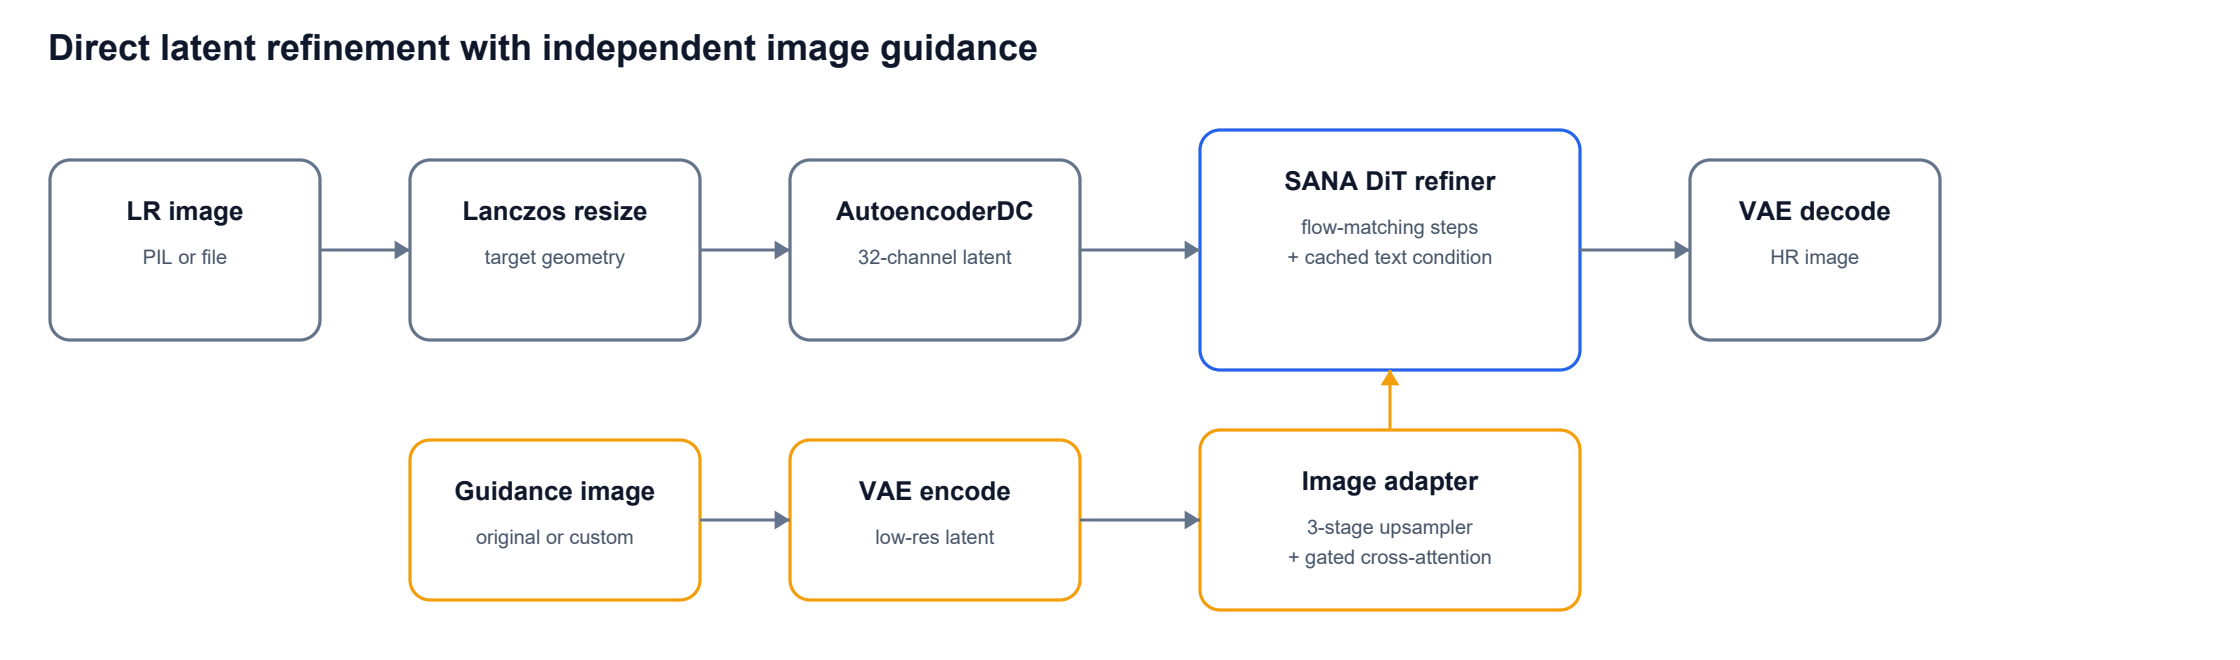
\includegraphics[width=0.98\columnwidth]{figures/architecture.png}
  \caption{\textbf{\method overview.} The input is resized to the requested
  output geometry and encoded into the latent state refined by a SANA DiT. A
  separate encoding of the original or user-provided guidance image is
  upsampled by a three-stage adapter and injected through gated attention.
  Cached text tensors remove the text encoder from the runtime.}
  \label{fig:architecture}
\end{figure}

\section{Method}
\label{sec:method}

\subsection{Direct latent refinement}

Let the requested enlargement factor be $s\in\{2,4,8\}$. We first resize the
input to the padded target geometry:
\begin{equation}
  \widetilde{\bm{x}} =
  \mathcal{R}_{s}\!\left(\bm{x}_{\mathrm{LR}}\right),
\end{equation}
where $\mathcal{R}_{s}$ is Lanczos by default and padding makes both dimensions
compatible with the VAE stride. The VAE encoder $\mathcal{E}$ produces the
target-sized latent
\begin{equation}
  \bm{z}_{0} = \mathcal{E}(\widetilde{\bm{x}})\in
  \R^{B\times 32\times H_z\times W_z}.
\end{equation}
Unlike a noise-initialized image-generation pipeline, \method retains
$\bm{z}_{0}$ as the initial state; no Gaussian noise is added at inference.
A flow-matching transformer predicts the update field at a sequence of
effective refinement levels
$\{\sigma_k\}_{k=1}^{K}$. For the linear schedule used in the reported
experiments,
\begin{equation}
  \sigma_k =
  \sigma_{\max} -
  \frac{k-1}{K-1}
  \left(\sigma_{\max}-\frac{\sigma_{\max}}{K}\right),
\end{equation}
with the one-step case defined simply as $\sigma_1=\sigma_{\max}$. The runtime
unshifts these effective values according to the checkpoint scheduler and
appends the terminal value $\sigma_{K+1}=0$. Each FlowMatch Euler update is
\begin{equation}
  \bm{z}_{k+1}=\bm{z}_{k}
  +(\sigma_{k+1}-\sigma_k)\,
  \bm{v}_{\theta}(\bm{z}_{k},\sigma_k,\bm{z}_{g},s).
\end{equation}
At inference the unknown clean component of the training interpolation path
cannot be constructed, so the resized-image latent is used directly as the
initial estimate. Consequently, $\sigma_{\max}$ acts as a refinement step
size rather than asserting that the initial state is an exact sample from the
training path.

\subsection{SANA transformer backbone}

The transformer extends the SANA Diffusion Transformer implementation. It
keeps the linear-attention backbone, timestep-conditioned adaptive
normalization, text cross-attention, and flow-matching output head, while
adding an image-guidance path. The released implementation accepts 32-channel
VAE latents. The scale $s$ is supplied to the transformer so that one
checkpoint can process all three enlargement factors.

Text remains useful as a weak prior even when the input image supplies most
semantic information. Rather than loading a language model or text encoder at
runtime, the checkpoint stores embeddings and masks for a fixed positive
description and an empty prompt. When classifier-free guidance is disabled
($w\leq 1$), only the positive condition is evaluated. For $w>1$, the
unconditional and conditional predictions are combined as
\begin{equation}
  \bm{v} = \bm{v}_{u} + w(\bm{v}_{c}-\bm{v}_{u}).
\end{equation}

\subsection{Image-guidance adapter}
\label{sec:adapter}

The default guidance observation is the original input, although a separate
image can be supplied. It is resized to the unscaled padded geometry, encoded
with the same VAE, and multiplied by a conditioning strength $\alpha$:
\begin{equation}
  \bm{z}_{g} = \alpha\,
  \mathcal{E}\!\left(\mathcal{R}_{1}(\bm{x}_{g})\right).
\end{equation}
The adapter maps $\bm{z}_{g}$ to target latent resolution using a $3\times3$
input convolution followed by up to three learned $2\times$ upsampling stages.
Each stage contains two residual convolutions, bilinear interpolation, and a
post-convolution. The number of active stages is $\log_2 s$.

The resulting guidance map is projected to the transformer's inner dimension.
By default, every second transformer block performs cross-attention from the
image tokens to these guidance tokens. Its output passes through a
zero-initialized, timestep-conditioned gate before addition to the main
residual stream. A second zero-initialized adaptive $1\times1$ convolution
injects guidance into the first feed-forward feature map. Zero initialization
lets the adapter begin as a no-op relative to the pretrained transformer and
learn its contribution during fine-tuning.

\subsection{Tiled inference}
\label{sec:tiling}

Large images require distinct strategies for the autoencoder and transformer.
For the VAE we call the native \texttt{AutoencoderDC.enable\_tiling} mechanism
with a default sample tile of 1024 pixels and overlap of 256 pixels. We do not
wrap this in another spatial tiler, because an outer blending coordinate system
can disagree with native VAE crop geometry.

The DiT is tiled independently in latent space. Given latent tile size $T$ and
overlap $O$, each tile produces an updated latent $\widehat{\bm{z}}_i$. A
separable Hann window $\bm{W}_i$, clamped elementwise to a minimum of
$10^{-3}$ so that outer image edges retain non-zero support, blends all
predictions:
\begin{equation}
  \bm{z}^{k+1} =
  \frac{\sum_i \bm{W}_i\odot\widehat{\bm{z}}_i^{k+1}}
       {\sum_i \bm{W}_i+\epsilon}.
\end{equation}
The accumulated weights are normalized with a minimum denominator of
$10^{-6}$. Every tile reads from the same globally assembled latent for a
given step. On alternate steps after the first, the grid is shifted by half a
stride so that boundaries do not remain fixed across the trajectory.
Accumulation and weights use FP32, while VAE and transformer passes use the
checkpoint dtype.

Tile batches are selected from available accelerator memory, capped at 16
tiles, and reduced by half following CUDA out-of-memory errors. Classifier-free
guidance is included in this memory estimate because it doubles the model
batch.

\subsection{Progressive training curriculum}
\label{sec:training}

We did not change a text-to-image checkpoint into a direct refiner in a single
optimization run. The training curriculum progressively changes the data
distribution, conditioning mechanism, and finally the flow endpoints. All
stages are full-parameter updates rather than LoRA training. The curriculum is
summarized in \cref{tab:curriculum}.

\begin{table*}[t]
  \centering
  \caption{Progressive curriculum leading to the released checkpoint. ``Mixed''
  denotes the v1 objective that retains the original noise endpoint while
  replacing the clean-side input by a degraded latent with probability 0.5.}
  \label{tab:curriculum}
  \small
  \begin{tabular}{p{0.17\textwidth}p{0.24\textwidth}p{0.25\textwidth}p{0.25\textwidth}}
    \toprule
    Stage & Initialization and trainable modules & Path / objective & Purpose\\
    \midrule
    Domain and schedule adaptation &
    Upstream SANA; all DiT parameters &
    Standard clean--noise flow matching on our curated images under the
    Z-Image schedule &
    Move the generative prior toward the target image distribution before
    asking it to restore LR observations.\\
    Adapter warm-up (v1 CPT) &
    Adapted SANA plus a new zero-initialized image branch; backbone and adapter
    jointly trainable &
    Mixed clean/degraded source with probability 0.5; conventional flow target &
    Learn multi-scale LR conditioning without abruptly discarding the
    generative behavior.\\
    Adapter SFT &
    v1 milestone 10,000; all transformer and adapter parameters &
    Same mixed path on a stricter quality-filtered subset without the retained
    defect subset &
    Consolidate restoration and conditioning on cleaner targets; checkpoint
    6,000 initializes the released final stage.\\
    Direct refinement &
    v1-SFT checkpoint 6,000; all transformer and adapter parameters &
    100\% degraded-to-clean latent path plus pixel and high-frequency losses &
    Match the short refinement trajectory used by the public runtime.\\
    \bottomrule
  \end{tabular}
\end{table*}

\paragraph{Stage 1: adapting the SANA prior.}
We first adapt all SANA DiT parameters to our curated image distribution and
the Z-Image/FLUX-style flow schedule (shift 3, 1,000 training timesteps).
The broad CPT phase includes a wider quality range and deliberately retained
defect examples; subsequent SFT uses cleaner, more caption-aligned data. This
stage contains no image-guidance adapter. Its role is to shift the image prior
and flow behavior before introducing the structurally different
super-resolution task.

\paragraph{Stages 2--3: introducing and stabilizing image guidance.}
We then attach the adapter described in \cref{sec:adapter}. Its residual gates
and first-block feed-forward injection are initialized to zero, so the new
branch initially leaves the adapted backbone unchanged. The 256-channel
guidance encoder, three scale-dependent upsampling stages, ten image
cross-attention modules (one in every second block of the 20-block DiT), and
the complete SANA backbone are optimized jointly.

For a clean latent $\bm{z}_{\mathrm{HR}}$, Gaussian noise
$\bm{\epsilon}$, and Bernoulli variable $b\sim\mathrm{Bernoulli}(0.5)$, the
v1 stages use
\begin{align}
  \bm{z}_{\mathrm{src}} &=
  \begin{cases}
    \bm{z}_{\mathrm{deg}}, & b=1,\\
    \bm{z}_{\mathrm{HR}}, & b=0,
  \end{cases}\\
  \bm{z}_{\sigma}^{\mathrm{mixed}}
    &= (1-\sigma)\bm{z}_{\mathrm{src}}+\sigma\bm{\epsilon},\\
  \bm{v}^{*}_{\mathrm{mixed}}
    &= \bm{\epsilon}-\bm{z}_{\mathrm{HR}}.
\end{align}
Thus half of the examples expose the backbone to a target-sized degraded
latent while the target retains the conventional clean-to-noise flow field.
Independently, the adapter always receives the true low-resolution latent and
the selected scale. This mixed stage teaches the new image path while
preserving a generative fallback. The v1 SFT stage then resumes from v1
milestone 10,000, raises the quality threshold to 0.8, removes the retained
defect subset,
and retains the 0.5 mixture. We select its checkpoint 6,000 for the final
stage.

\paragraph{Stage 4: changing the target to direct refinement.}
The final stage changes the problem rather than merely continuing SFT.
For every example, an area-downsampled crop supplies the guidance image;
random bilinear or bicubic interpolation produces
$\bm{z}_{\mathrm{deg}}$ at target size. Factors $2$, $4$, and $8$ are sampled
uniformly. With \texttt{refine\_flow: direct} and degraded-input probability
1.0, training uses
\begin{align}
  \bm{z}_{\sigma}^{\mathrm{direct}}
    &= (1-\sigma)\bm{z}_{\mathrm{HR}}
       +\sigma\bm{z}_{\mathrm{deg}},\\
  \bm{v}^{*}_{\mathrm{direct}}
    &= \bm{z}_{\mathrm{deg}}-\bm{z}_{\mathrm{HR}}.
\end{align}
The model therefore learns the same degraded-to-clean direction traversed by
short-step inference, rather than a full noise-to-image generation path.

The predicted clean latent
$\widehat{\bm{z}}_{\mathrm{HR}}=
\bm{z}_{\sigma}^{\mathrm{direct}}-\sigma\bm{v}_{\theta}$ is decoded at
512 pixels. The final scalar objective is
\begin{equation}
\begin{split}
  \mathcal{L} =
  \underbrace{\operatorname{MSE}
  (\bm{v}_{\theta},\bm{v}^{*}_{\mathrm{direct}})}
  _{\mathcal{L}_{\mathrm{flow}}}
  +0.3\underbrace{\lVert\widehat{\bm{x}}_{\mathrm{HR}}
  -\bm{x}_{\mathrm{HR}}\rVert_1}_{\mathcal{L}_{\mathrm{recon}}}\\
  {}+0.5\underbrace{\lVert\Delta\widehat{\bm{x}}_{\mathrm{HR}}
  -\Delta\bm{x}_{\mathrm{HR}}\rVert_1}_{\mathcal{L}_{\mathrm{HF}}}\;,
  \end{split}
\end{equation}
where $\widehat{\bm{x}}_{\mathrm{HR}}$ is the frozen VAE-decoder output and
$\Delta$ is the normalized $3\times3$ Laplacian response. Gradients pass
through the decoder to the transformer and adapter, but decoder parameters
remain frozen throughout the reported stage.

Optimization uses AdamW with learning rate $2\times10^{-5}$, weight decay
0.01, BF16 precision, DeepSpeed ZeRO-2, gradient clipping at 2.0, and an
effective optimizer batch of 96. Training examples use 1024-pixel crops
decoded from source images at up to 2048 pixels. The final-stage split reserves
1\% for validation, applies 7.5\% prompt dropout, and conditionally adds an
image-type tag to the fixed prompt. The VAE and text encoders remain frozen;
only the transformer--adapter module receives optimizer updates. Process
allocation, cache production, seeds, validation cadence, and stage-boundary
state are reported in \cref{app:implementation}.

\section{Training Data Pipeline}
\label{sec:data}

Extreme super-resolution depends on high-frequency evidence in the training
targets. A nominally high-resolution image that is blurred, previously
upscaled, or heavily compressed teaches the model the wrong reconstruction
prior. We therefore built a metadata-first pipeline that profiles images at
native resolution and preserves content diversity while filtering technical
defects.

\begin{figure}[H]
  \centering
  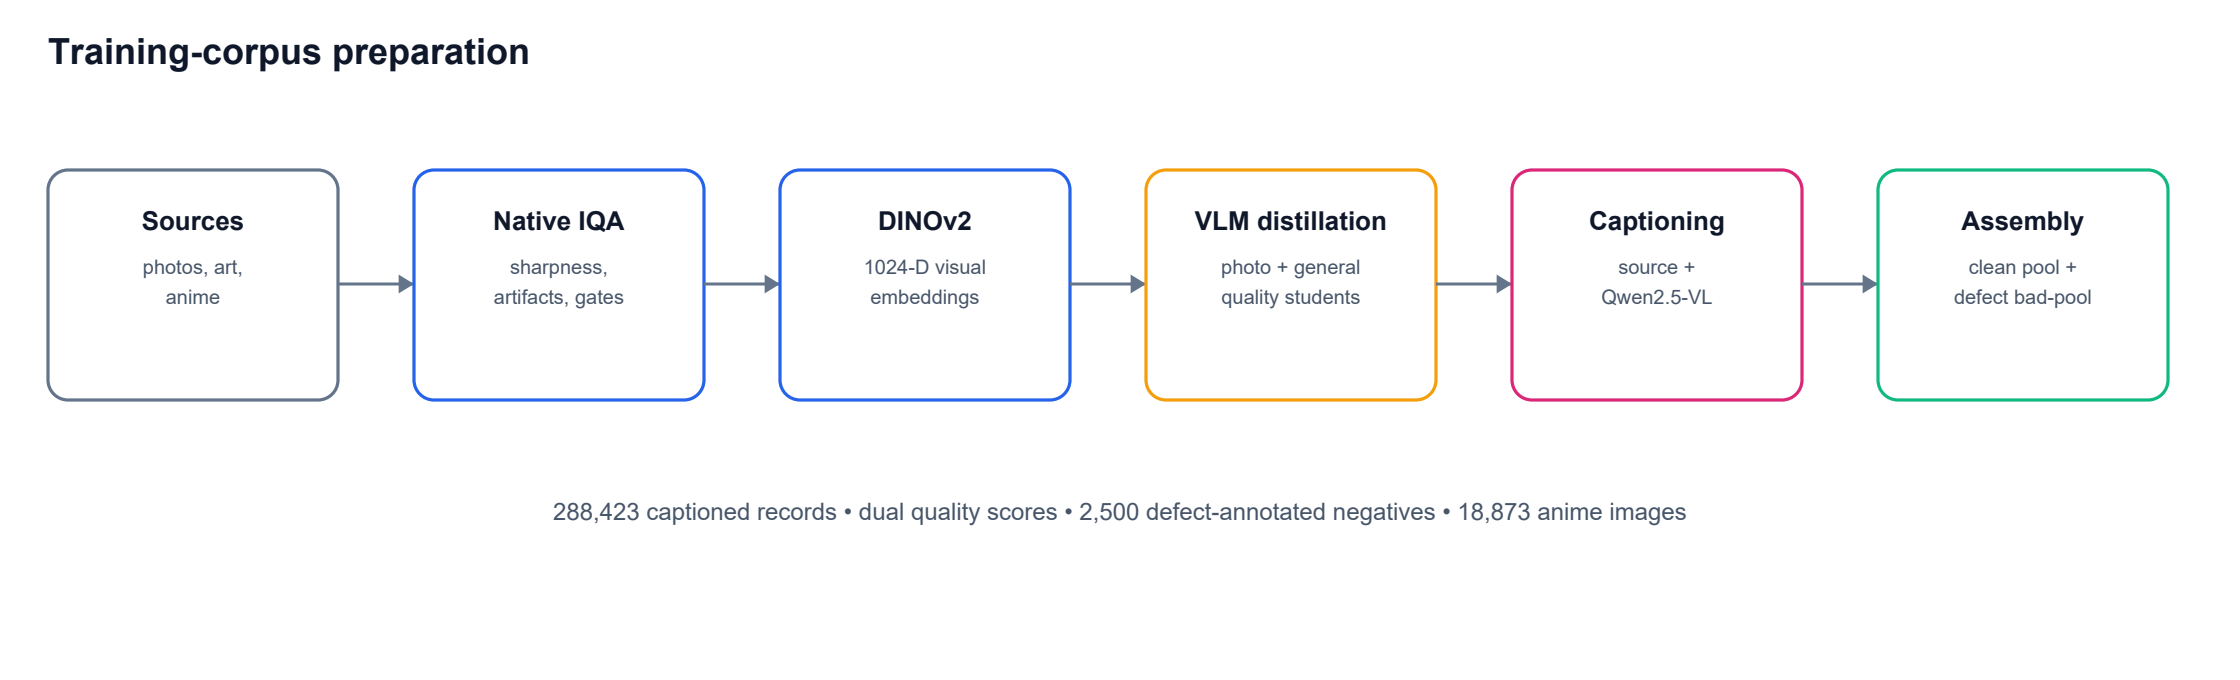
\includegraphics[width=0.98\columnwidth]{figures/data_pipeline.png}
  \caption{\textbf{Data pipeline.} Native-resolution measurements and DINOv2
  embeddings feed two VLM-distilled student quality models. Deterministic gates,
  captions, and a deliberately retained defect pool produce a training-ready
  corpus without copying the source images.}
  \label{fig:data_pipeline}
\end{figure}

\subsection{Sources and native-resolution profiling}

The final metadata index contains 288,423 records from CommonCatalog, PD12M,
4KLSDB, Unsplash, DIV8K, a small curated and synthetic fine-t2i set, and three
high-resolution SFW anime sources (yande, konachan, and danbooru). The pipeline
stores source references and derived metadata rather than duplicating the
image corpus.

Each image is decoded at native resolution. Measurements include JPEG
block-edge energy, a downsample--upsample Laplacian ratio, flat-patch noise,
local and global Laplacian statistics, Tenengrad, spectral slope,
high-frequency energy, edge density, JPEG quantization estimates, bytes per
pixel, borders, saturation, grayscale status, and a perceptual hash. The
down--up ratio was the most useful blur/prior-upscale detector and achieved
approximately 0.992 AUC on a labelled validation set. In a diagnostic CommonCatalog sample, 72\% of images triggered at least one native-resolution super-resolution flag that had been missed by the earlier thumbnail test.

\subsection{VLM-distilled scoring}

We extract the CLS embedding from DINOv2-large~\cite{oquab2024dinov2} after a
224-pixel resize. A photo-quality VLM rubric is informative for photographic
content but systematically penalizes illustration. We therefore collect two
teacher label sets: approximately 21k photo-rubric labels and 7.3k
content-agnostic labels under a fixed annotation budget.

Two small multi-layer perceptrons consume the DINOv2 embedding concatenated with standardized pixel features. Each has a scalar quality head and a watermark/overlay head. The photo student reaches Spearman $\rho\approx0.60$ against its teacher; the content-agnostic student reaches $\rho\approx0.36$. Although imperfect as absolute quality estimators, the two scores are inexpensive to evaluate over the full corpus and expose different domain biases.

\subsection{Gates, captions, and assembly}

Three universal gates flag extreme blockiness, softness, and noise. Additional photo-oriented gates for local sharpness, borders, over-compression, and low edge density are stored but disabled by default because they over-fire on flat-shaded art. The default base-corpus decision combines universal gates, overlay probability, and a general quality threshold of 60 on a 0--100 scale.

Existing source captions are reused where available. Missing short and long captions are generated by a local Qwen2.5-VL model~\cite{bai2025qwen25vl}.
Rather than discarding every low-scoring item, we uniformly sample 2,500
examples across the rejected score range. A VLM assigns one or more of 18
defect tags, and their captions explicitly state the defect. This retained
defect subset provides quality-conditioned negative examples.

Anime reveals a useful domain-shift case. The content-agnostic student model
rates the images reasonably, while photo-calibrated softness and low-detail
gates reject many valid flat-shaded illustrations. For the anime expansion we
therefore keep images based on the learned score and caption presence, without
the universal pixel gate. This yields 18,873 SFW anime records. Exact source
counts are reported in \cref{tab:dataset_sources}.

\section{Experiments}
\label{sec:experiments}

\subsection{Evaluation protocols}

\paragraph{Reference reconstruction.}
For each headline quality set, a known 512-pixel target is downsampled to 128
pixels with Lanczos and upscaled by a factor of four. We report RGB,
full-frame PSNR, SSIM, and MAE on a $[0,1]$ range; SSIM uses an $11\times11$
uniform window. The photo and anime sets each contain 12 public or externally
curated raster images. Bicubic and Lanczos resize the saved low-resolution
inputs directly to the target size and therefore act as deterministic,
protocol-matched interpolation baselines. All methods in a shared table
receive the same inputs.

\method uses the evaluated reconstruction preset: one refinement step,
$\sigma_{\max}=0.35$, guidance scale 1, BF16, and VAE tiling. The
same settings are used for the ablation below, so
\cref{tab:photo_quality,tab:full_ablation} differ only by runtime caching
details. We compute 95\% percentile bootstrap confidence intervals over images
with 10,000 resamples. The intervals are reported in \cref{app:bootstrap};
per-image values are provided in
\path{paper/data/revision/controlled_x4_12_per_image.csv} and
\path{paper/data/revision/revision_benchmarks.json}.

\paragraph{Expanded multi-scale reconstruction.}
A separate matrix uses 48 external photographs with 2048-pixel center-crop
targets and Lanczos-downsampled inputs at $2\times$, $4\times$, and $8\times$.
It uses the same one-step \method preset and the same interpolation and metric
implementations. This matrix evaluates scale behavior but is not pooled with
the two 12-image headline sets.

\paragraph{Latency.}
All timing uses an NVIDIA GeForce RTX 5090 with models already resident in
VRAM. Each cell includes 24 images, three warm-up calls per image and ten timed
calls, for 240 calls. The interval covers PIL file open, preprocessing, VAE
encoding when applicable, inference, and final image conversion. Model loading
and output-file writing are excluded. Native JPEG sizes can be much larger than
the 1024-pixel output, so the values are end-to-end file-processing latency.
Real-ESRGAN is natively $4\times$; its output is resized for requested
$2\times$ and $8\times$ conditions.

\paragraph{Ablation.}
Prompt and image-adapter components are evaluated on 12 photographs at
128-to-512 $4\times$ reconstruction with one refinement step,
$\sigma_{\max}=0.35$, guidance scale 1, and BF16. Latent caches are disabled
and every configuration receives the same images. Exact deterministic settings
are listed in \cref{app:implementation}.

\subsection{Training trace}

The final direct-refinement run lasted 49,006 s (13 h 36 min 46 s). Peak
allocated GPU memory was
21.77 GB. Validation loss decreased from 0.1954 at update 100 to 0.1452 at
update 4,000, a 25.69\% relative reduction. Machine-readable provenance and milestone
values are included in \texttt{paper/data/training\_run.json}.

\begin{figure}[H]
  \centering
  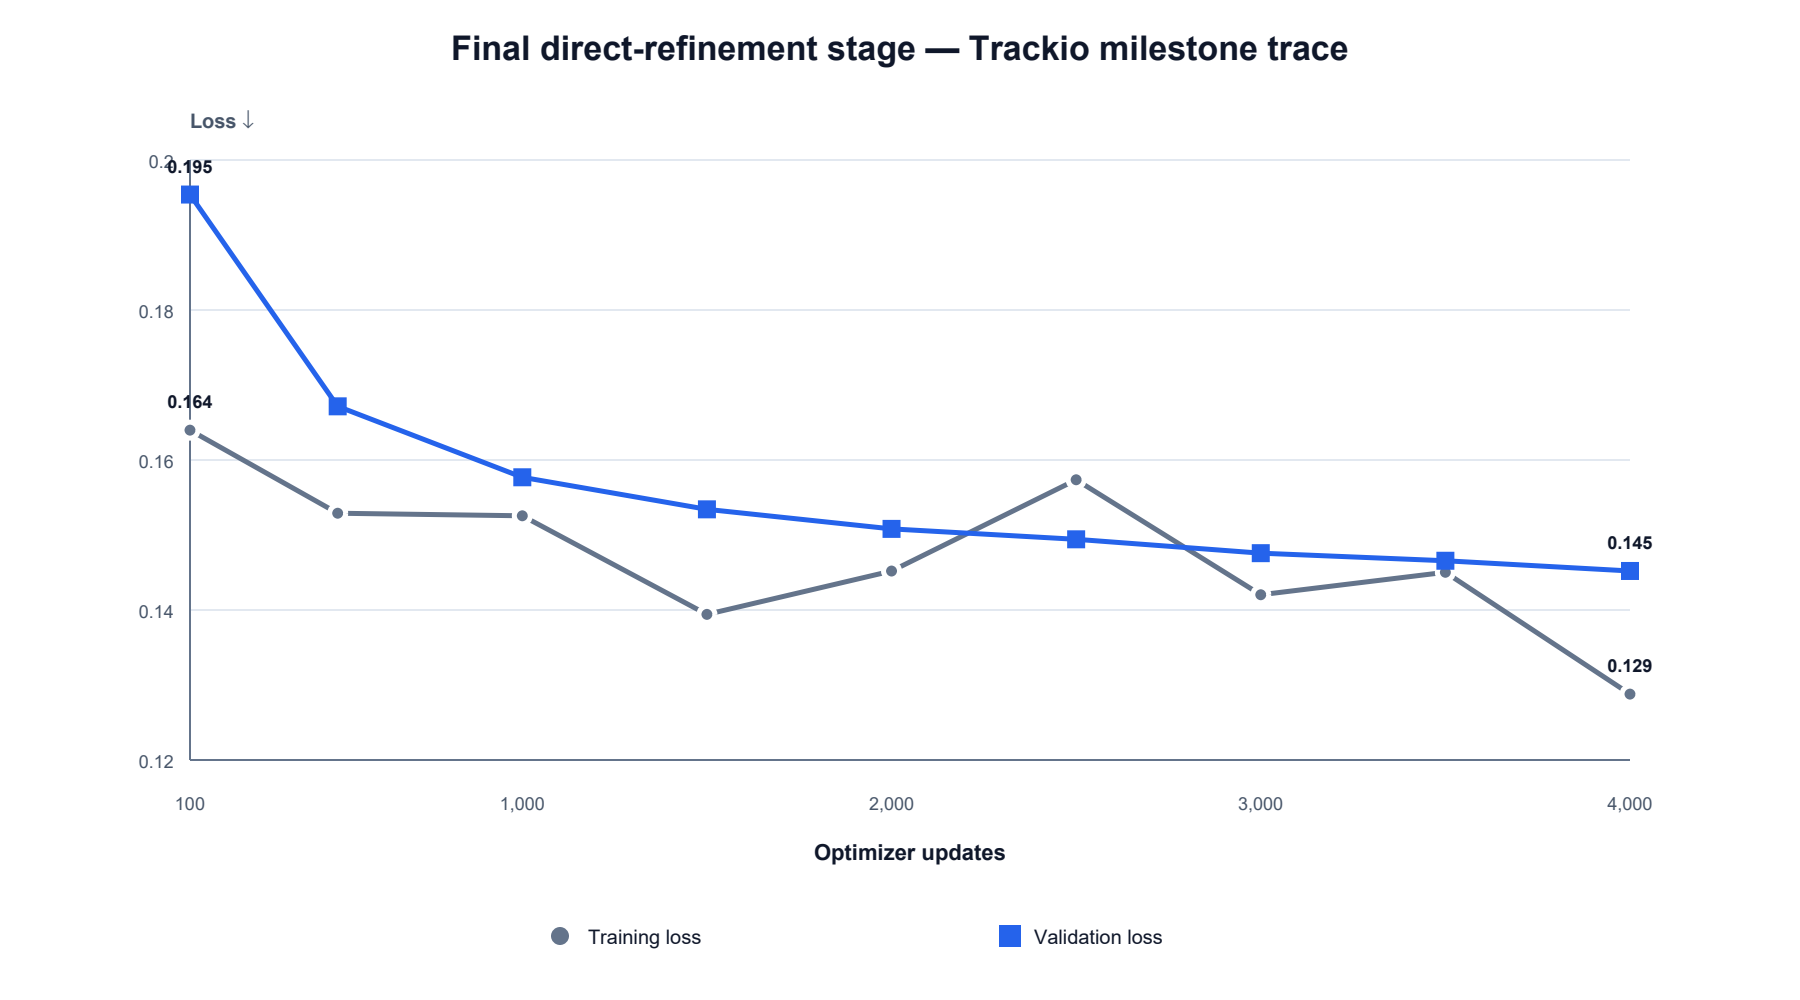
\includegraphics[width=\columnwidth]{figures/training_curve.png}
  \caption{Trackio milestones from the final 4,000-update direct-refinement
  stage. Training loss is a stochastic per-update measurement; validation is
  evaluated every 100 updates, with selected milestones shown here.}
  \label{fig:training_curve}
\end{figure}

\subsection{Controlled reconstruction}

\begin{table}[H]
  \centering
  \caption{Shared $4\times$ photo reconstruction set (12 images). Interpolation
  baselines are evaluated on the saved Lanczos-downsampled inputs.}
  \label{tab:photo_quality}
  \small
  \begin{tabular}{lccc}
    \toprule
    Method & PSNR $\uparrow$ & SSIM $\uparrow$ & MAE $\downarrow$\\
    \midrule
    Lanczos & \textbf{33.4340} & \textbf{0.8308} & \textbf{0.01910}\\
    Bicubic & 33.2358 & 0.8248 & 0.01943\\
    \method & 31.8170 & 0.7877 & 0.02314\\
    Real-ESRGAN & 29.6409 & 0.7587 & 0.02846\\
    LUA & 19.5536 & 0.4071 & 0.09247\\
    \bottomrule
  \end{tabular}
\end{table}

\begin{table}[H]
  \centering
  \caption{Shared $4\times$ anime reconstruction set (12 images). Interpolation
  baselines are evaluated on the saved Lanczos-downsampled inputs.}
  \label{tab:anime_quality}
  \small
  \begin{tabular}{lccc}
    \toprule
    Method & PSNR $\uparrow$ & SSIM $\uparrow$ & MAE $\downarrow$\\
    \midrule
    Lanczos & \textbf{28.7939} & 0.8650 & \textbf{0.02184}\\
    Bicubic & 28.3830 & 0.8614 & 0.02190\\
    \method & 28.4394 & 0.8560 & 0.02382\\
    Real-ESRGAN & 26.7850 & \textbf{0.8695} & 0.02559\\
    LUA & 17.2268 & 0.3653 & 0.10970\\
    \bottomrule
  \end{tabular}
\end{table}

\Cref{tab:photo_quality,tab:anime_quality} separate two comparisons. Among the
learned methods, \method has the highest PSNR and lowest MAE on both sets,
including a 2.176 dB photo PSNR margin over Real-ESRGAN. The interpolation
baselines, however, retain more reference pixels: Lanczos leads photo PSNR by
1.617 dB and anime PSNR by 0.355 dB over \method. This is expected because the
inputs themselves are produced by Lanczos and interpolation does not synthesize
new texture that can be penalized by paired distortion metrics. The 95\%
bootstrap intervals are wide and overlapping on these small sets. Real-ESRGAN
retains the highest anime SSIM, further illustrating that no single metric
defines the ranking.

\begin{table}[H]
  \centering
  \caption{Separate multi-scale reconstruction matrix on 48 external
  photographs with 2048-pixel targets. All rows use the same target crops and
  Lanczos-downsampled inputs.}
  \label{tab:multiscale48}
  \small
  \begin{tabular}{llccc}
    \toprule
    Scale & Method & PSNR $\uparrow$ & SSIM $\uparrow$ & MAE $\downarrow$\\
    \midrule
    \multirow{3}{*}{$2\times$}
      & Lanczos & \textbf{36.6473} & \textbf{0.9120} & \textbf{0.01287}\\
      & Bicubic & 36.1985 & 0.9059 & 0.01336\\
      & \method & 30.2797 & 0.7641 & 0.02451\\
    \midrule
    \multirow{3}{*}{$4\times$}
      & Lanczos & \textbf{32.0484} & \textbf{0.8221} & \textbf{0.01973}\\
      & Bicubic & 31.8412 & 0.8168 & 0.02000\\
      & \method & 30.7892 & 0.7875 & 0.02272\\
    \midrule
    \multirow{3}{*}{$8\times$}
      & Lanczos & \textbf{29.2018} & \textbf{0.7348} & \textbf{0.02532}\\
      & Bicubic & 29.0510 & 0.7303 & 0.02556\\
      & \method & 29.1155 & 0.7336 & 0.02589\\
    \bottomrule
  \end{tabular}
\end{table}

At $8\times$, the \method PSNR gap to Lanczos narrows to 0.086 dB and
\method exceeds Bicubic by 0.064 dB; their confidence intervals overlap. At
$2\times$ and $4\times$, conservative interpolation retains a clear distortion
advantage. The matrix therefore supports multi-scale operation, but not
distortion-metric leadership over interpolation.

PiD is designed to synthesize high-resolution pixel detail from latent
conditioning. We therefore exclude it from the 512-pixel headline tables: the
available public \texttt{PiD\_res2k\_sr4x} checkpoint targets roughly
2048-pixel outputs, and its archived 512-pixel results exhibit a regular
lattice artifact. The native-resolution experiment is reported
separately below.
LUA optimizes a different point again: a single feed-forward latent adapter
with scale-specific heads, which is inexpensive but is not trained to restore
the exact reference pixels of this protocol. The reported reconstruction gaps
for both methods should therefore not be interpreted as a general aesthetic
ranking; they quantify agreement with a known target under one protocol.

\begin{table}[H]
  \centering
  \caption{Native-resolution PiD $4\times$ photo reconstruction (12 real
  images). Each ground-truth target is a 2048-pixel crop from an original
  3--7K photograph and the input is its 512-pixel Lanczos downsample.}
  \label{tab:pid_native_quality}
  \small
  \begin{tabular}{lccc}
    \toprule
    Method & PSNR $\uparrow$ & SSIM $\uparrow$ & MAE $\downarrow$\\
    \midrule
    \textbf{\method} & \textbf{31.4801} & \textbf{0.8114} & \textbf{0.02061}\\
    Real-ESRGAN & 29.2505 & 0.7786 & 0.02571\\
    PiD (native 2k) & 26.1275 & 0.6683 & 0.03635\\
    LUA & \multicolumn{3}{c}{Flux-VAE OOM at 2048\,px (32\,GB)}\\
    \bottomrule
  \end{tabular}
\end{table}

At its intended 2048-pixel output, PiD no longer exhibits the regular lattice
artifact. Its reconstruction scores remain below \method and Real-ESRGAN on
this strict paired protocol, but they are valid measurements of the released
PiD checkpoint rather than an out-of-regime failure.

\subsection{Perceptual metrics}

\begin{table}[H]
  \centering
  \caption{Perceptual distances on the shared 512-pixel $4\times$ sets
  (12 images per domain; lower is better). LPIPS uses AlexNet and DISTS uses
  \texttt{piq}. Interpolation methods operate on the same saved LR inputs.
  PiD is omitted because its archived 512-pixel outputs are out of regime;
  LUA per-image outputs were not archived.}
  \label{tab:perceptual}
  \small
  \begin{tabular}{llcc}
    \toprule
    Domain & Method & LPIPS $\downarrow$ & DISTS $\downarrow$\\
    \midrule
    \multirow{4}{*}{Photo}
          & \method & 0.4221 & 0.1766\\
          & Real-ESRGAN & \textbf{0.3778} & 0.1950\\
          & Bicubic & 0.4551 & \textbf{0.1726}\\
          & Lanczos & 0.4718 & 0.1753\\
    \midrule
    \multirow{4}{*}{Anime}
          & \method & 0.2624 & \textbf{0.1215}\\
          & Real-ESRGAN & \textbf{0.1537} & \textbf{0.1215}\\
          & Bicubic & 0.2956 & 0.1253\\
          & Lanczos & 0.2927 & 0.1268\\
    \bottomrule
  \end{tabular}
\end{table}

\Cref{tab:perceptual} changes the interpretation of the distortion tables.
Lanczos no longer leads: on photo LPIPS it trails \method by 0.050 and on anime
LPIPS it trails by 0.030. Bicubic obtains the lowest photo DISTS, although its
95\% interval overlaps those of Lanczos and the learned methods are not
recomputed here with matched intervals. Real-ESRGAN remains best on LPIPS in
both domains, while \method is best or tied on anime DISTS. Thus no method
dominates both exact reconstruction and learned perceptual similarity.

\begin{figure}[H]
  \centering
  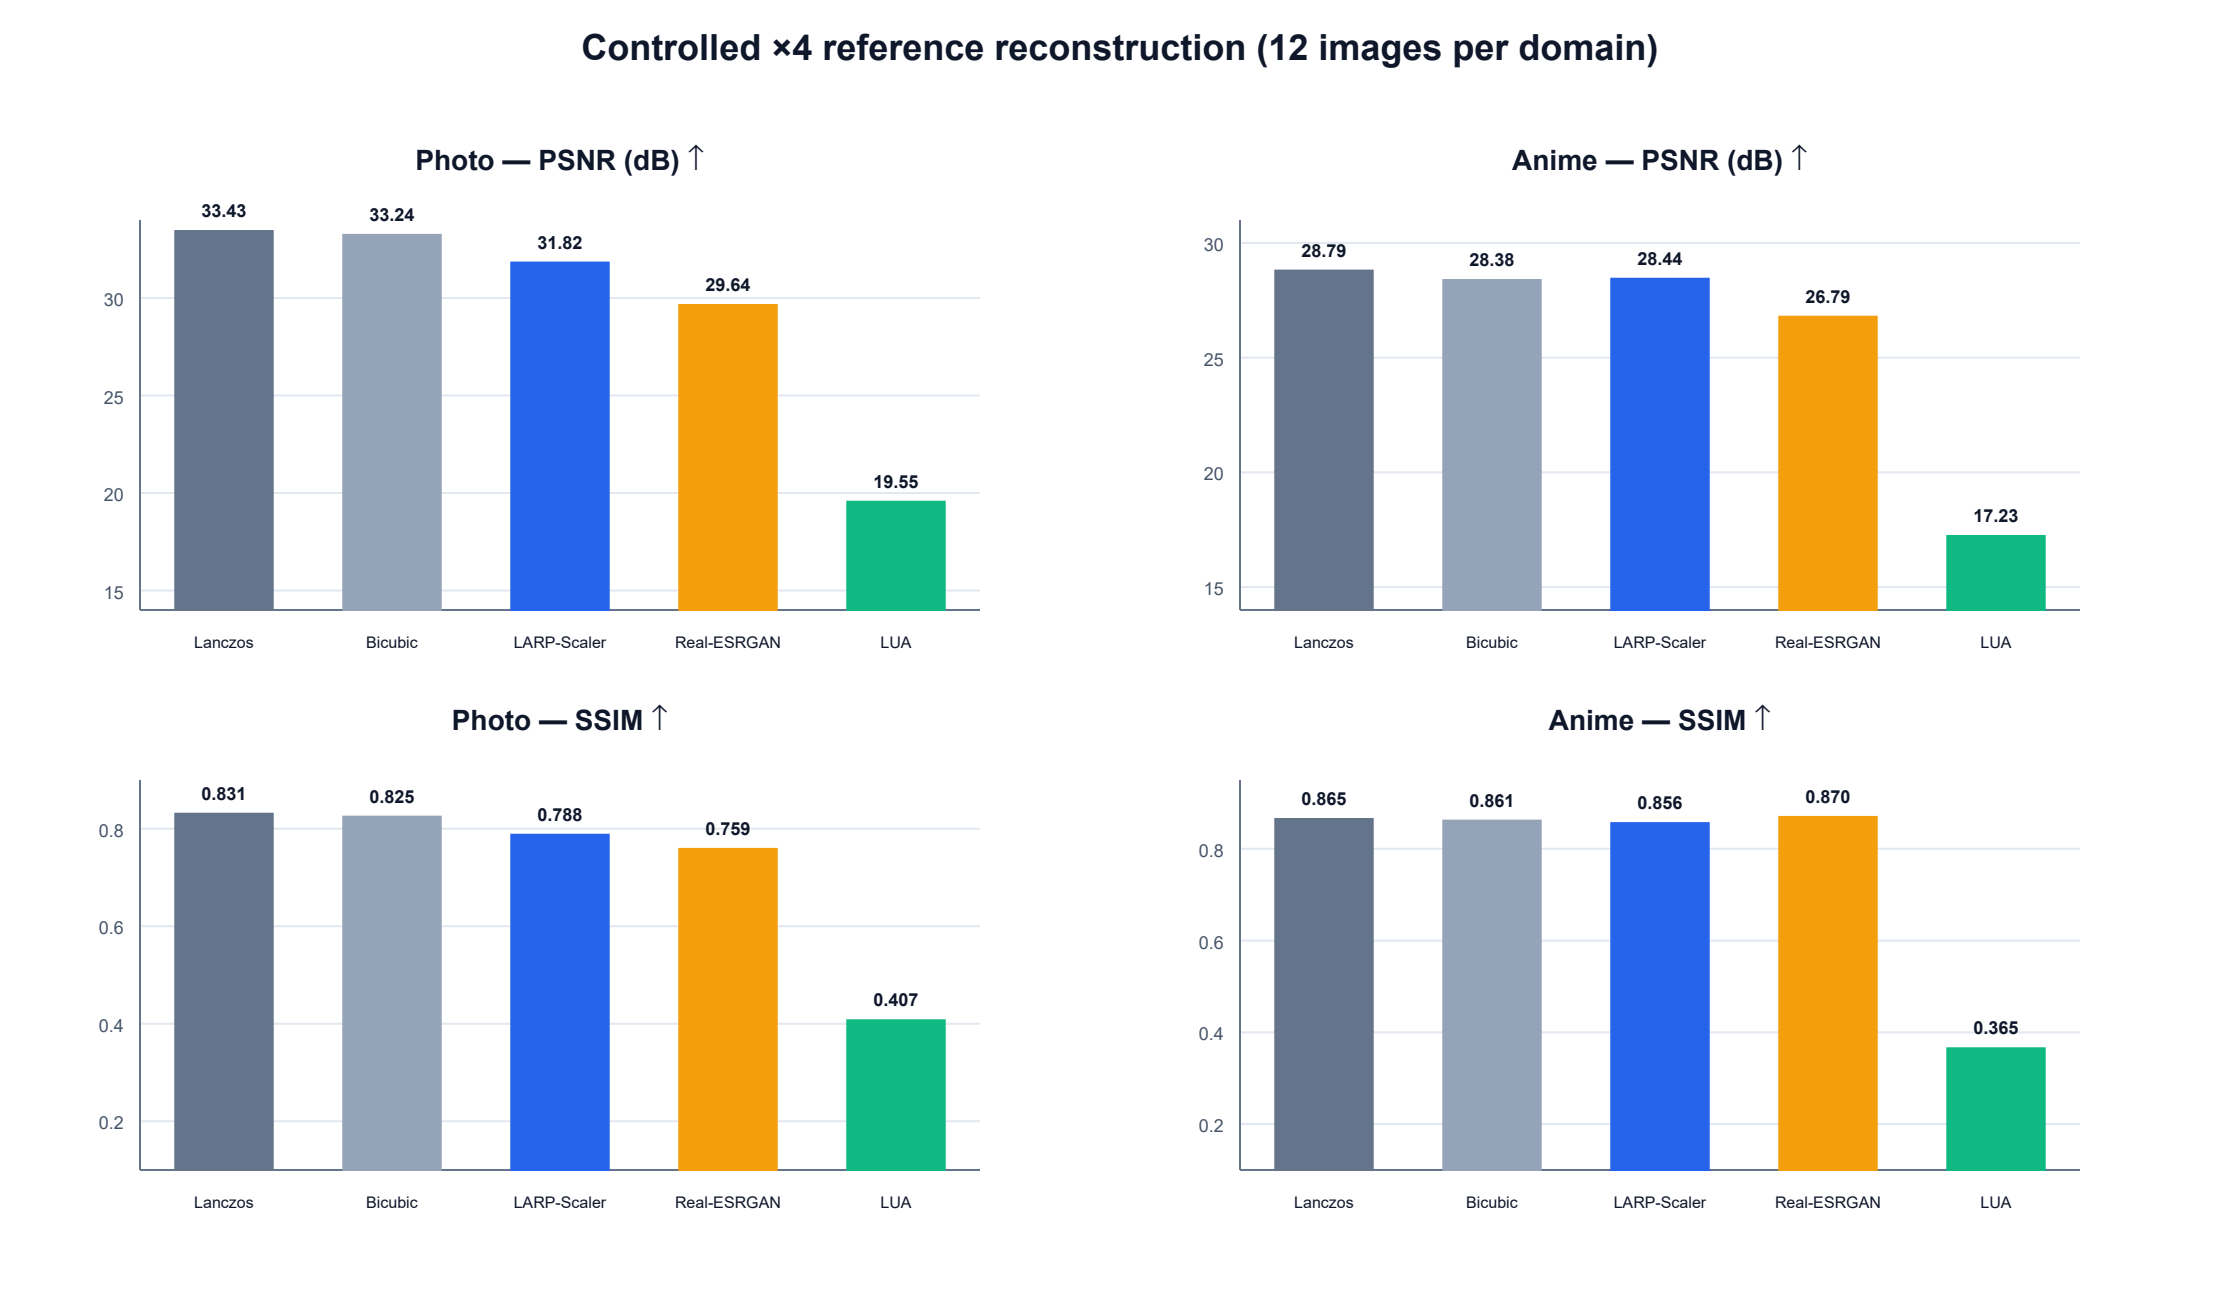
\includegraphics[width=0.96\columnwidth]{figures/quality_comparison.png}
  \caption{PSNR and SSIM on the controlled photo and anime reconstruction
  sets. Exact values and MAE are reported in
  \cref{tab:photo_quality,tab:anime_quality}.}
  \label{fig:quality}
\end{figure}

\subsection{Latency}

\begin{table}[H]
  \centering
  \caption{Median end-to-end latency in seconds for 1024-pixel output on 24
  photographs. Each cell aggregates 240 calls. Lower is better.}
  \label{tab:latency}
  \small
  \begin{tabular}{lccc}
    \toprule
    Method & $2\times$ & $4\times$ & $8\times$\\
    \midrule
    \method & \textbf{0.8119} & 0.8227 & 0.8047\\
    LUA & 2.6323 & \textbf{0.6291} & 0.6668\\
    Real-ESRGAN & 1.0253 & 0.6681 & \textbf{0.6134}\\
    \bottomrule
  \end{tabular}
\end{table}

The 1024-pixel PiD latency row is excluded because it uses the same 2k-native
checkpoint out of its intended output regime. At $4\times$, \method is 30.8\%
slower than LUA and 23.1\% slower than Real-ESRGAN. At $2\times$ it has the
lowest median in this protocol, while Real-ESRGAN is fastest at $8\times$.
Consequently, the evidence supports a competitive quality--latency trade-off,
not universal speed leadership.

\begin{table}[H]
  \centering
  \caption{Separate PiD latency measurement at its native
  $512\!\to\!2048$ $4\times$ operating point on three photographs. The model
  is loaded once; 3 warm-ups and 10 timed calls are run per image.}
  \label{tab:pid_native_latency}
  \small
  \begin{tabular}{lcccc}
    \toprule
    Method & Calls & Median (s) & Mean (s) & P10--P90 (s)\\
    \midrule
    PiD (native 2k) & 30 & 1.537 & 1.538 & 1.524--1.548\\
    \bottomrule
  \end{tabular}
\end{table}

\Cref{tab:pid_native_latency} restores the missing PiD speed measurement
without mixing resolutions. It includes input conversion, Flux-VAE encoding,
four PiD denoising steps, and CPU/PIL output conversion, but excludes model
loading and file writing. Peak allocated GPU memory was 19.34\,GiB on the
RTX~5090. Because the 1024-pixel table uses 24 different source photographs,
the native PiD row is reported separately rather than used for a direct speed
ranking.

\begin{figure}[H]
  \centering
  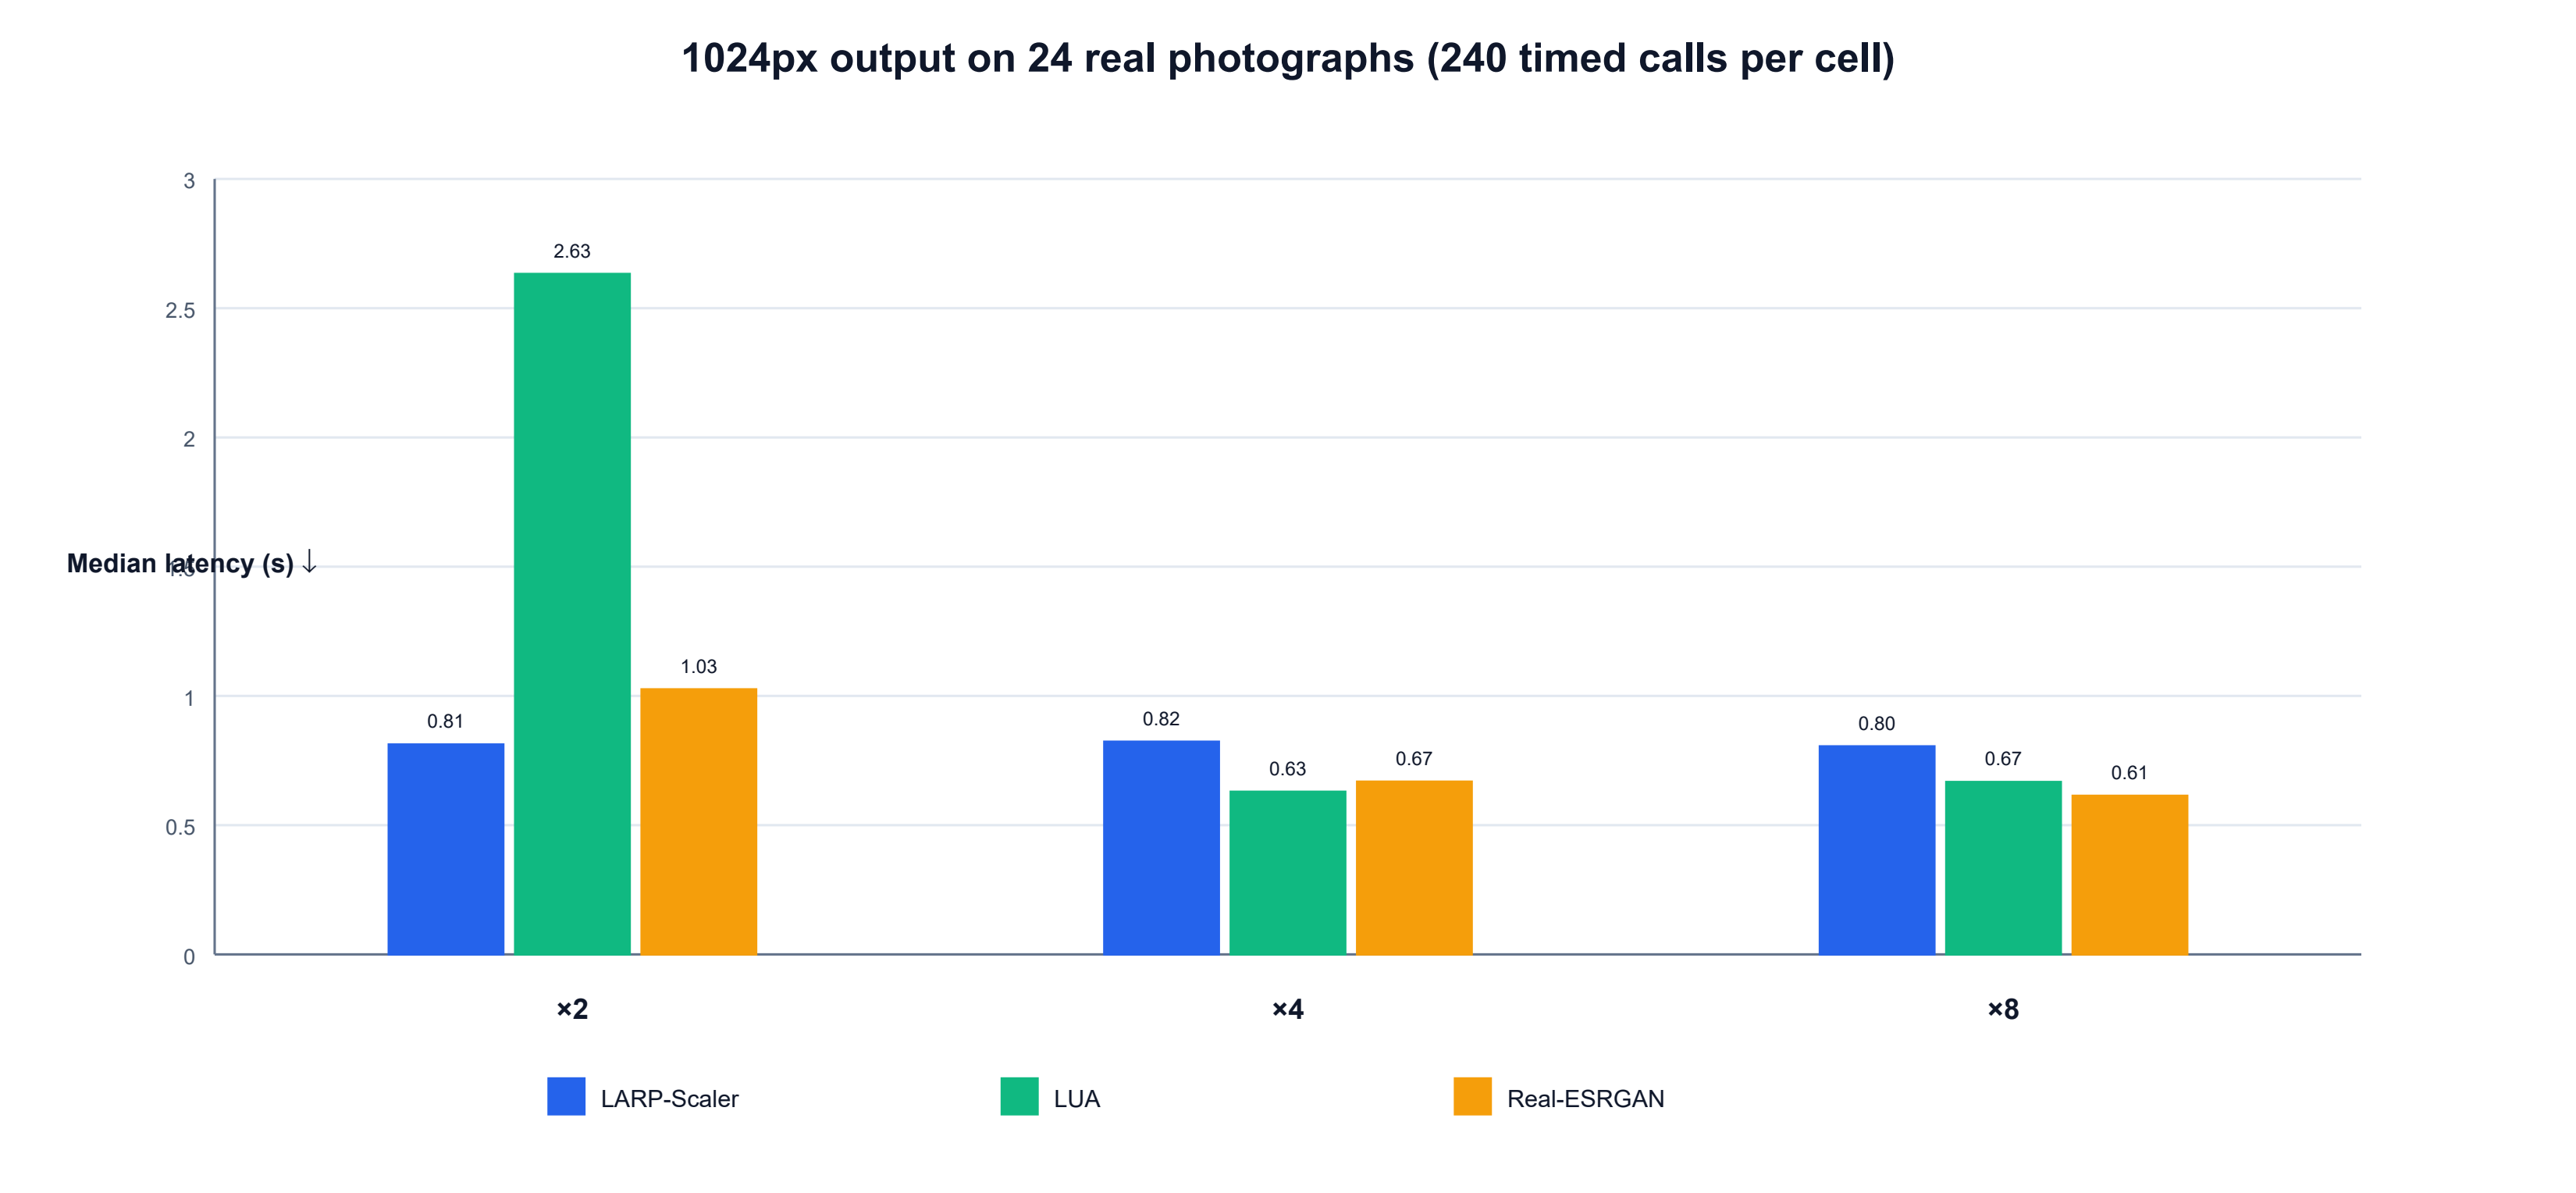
\includegraphics[width=0.88\columnwidth]{figures/latency_1024.png}
  \caption{Median end-to-end file-processing latency. The large LUA
  $2\times$ value illustrates why performance should be reported per scale
  rather than collapsed to a single average.}
  \label{fig:latency}
\end{figure}

\subsection{Prompt and adapter ablation}

\begin{table}[H]
  \centering
  \caption{Selected ablation changes on 12 photographs. MSE reduction is
  computed from $\Delta$PSNR as $1-10^{-\Delta/10}$.}
  \label{tab:ablation}
  \small
  \begin{tabular}{lrr}
    \toprule
    Change & $\Delta$PSNR & MSE red.\\
    \midrule
    Detailed prompt, adapter off & +0.0166 & 0.38\%\\
    Detailed prompt, adapter on & +0.0057 & 0.13\%\\
    Adapter branch, tagged prompt & \textbf{+0.5138} & \textbf{11.16\%}\\
    Matched vs.\ mismatched guidance & +0.0788 & 1.80\%\\
    \bottomrule
  \end{tabular}
\end{table}

Measured on the same 12 photographs and the same one-step protocol, the
released checkpoint improves on the untrained SANA backbone by 10.555 dB
(21.2628 to 31.8178 dB in the tagged-prompt, matched-guidance configuration;
see \cref{tab:full_ablation}). That gap is the combined effect of the
direct-refinement training stage and the guidance branch, and unlike the
cross-protocol comparison in \cref{app:extra} it is measured on identical
inputs.

Enabling the trained adapter branch is the largest measured architectural
change within the released system: in the tagged-prompt configuration it
raises PSNR from 31.3040 to 31.8178 dB. Replacing mismatched guidance by the
matched low-resolution image accounts for only 0.0788 dB. This suggests a
measurable but small content-specific contribution under this protocol; the
larger branch-on difference should not be attributed entirely to matched image
content. Prompt gains are positive but small and shrink after the adapter is
enabled.

\begin{figure}[H]
  \centering
  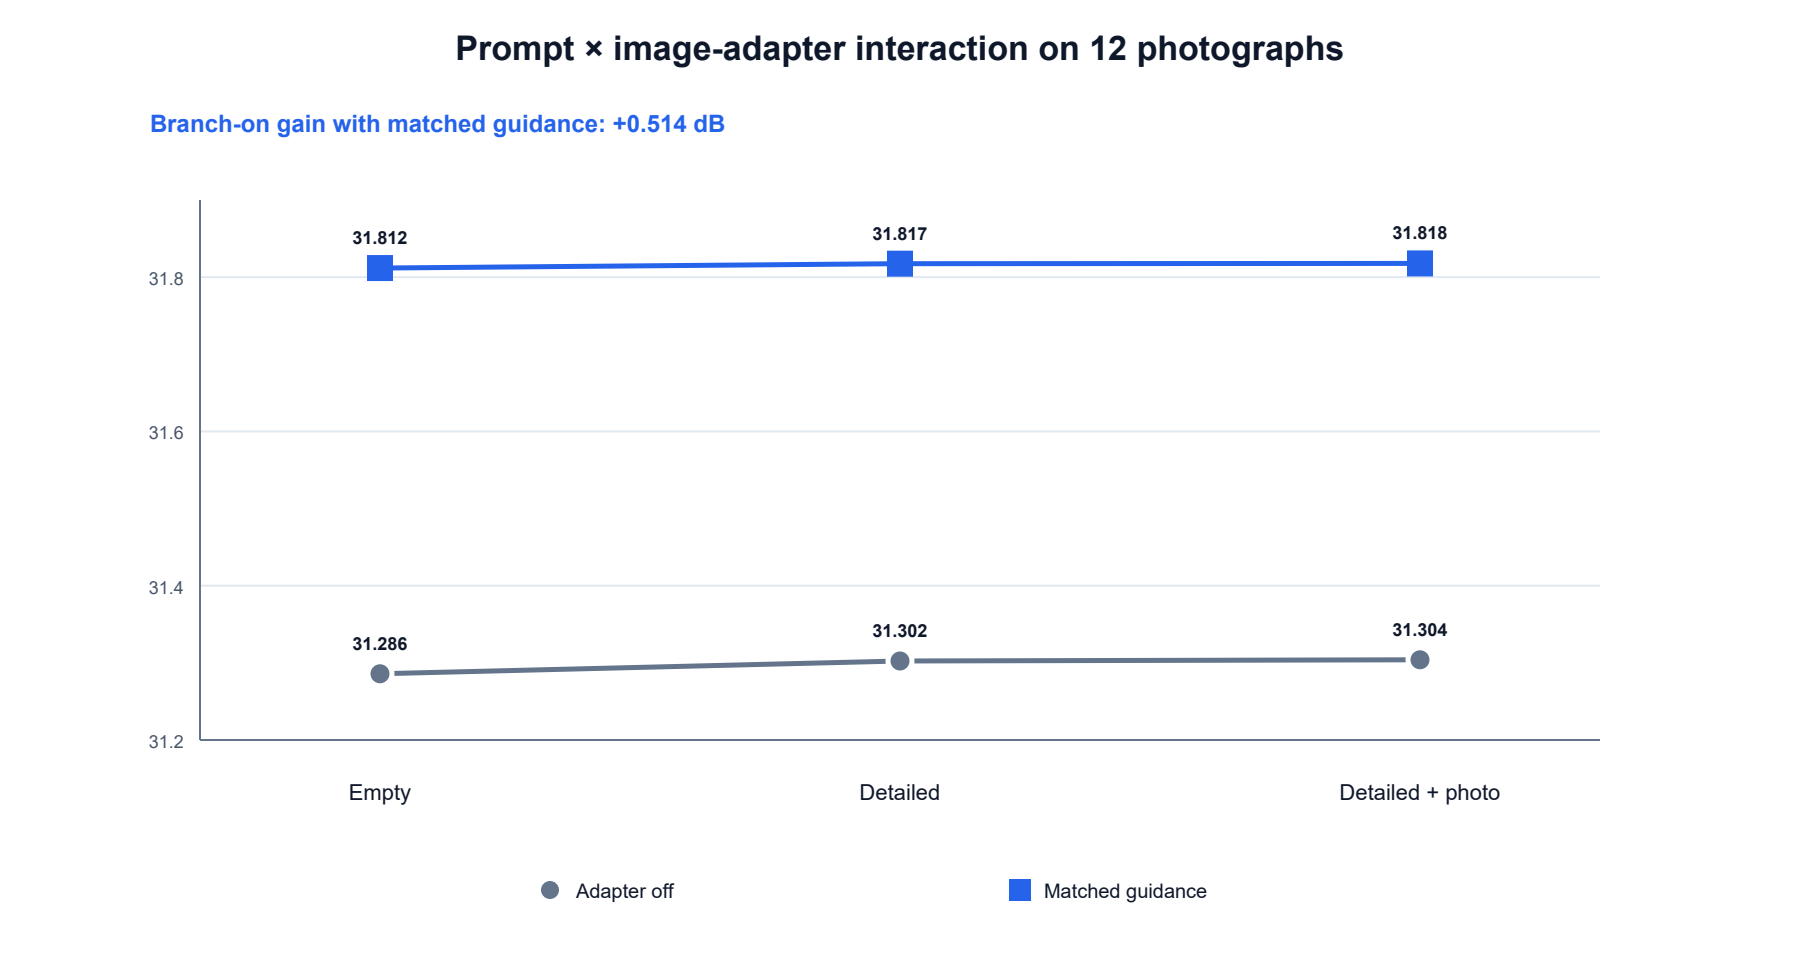
\includegraphics[width=\columnwidth]{figures/prompt_adapter_ablation.png}
  \caption{Prompt--adapter interaction. The y-axis is intentionally narrow to
  expose the prompt effect; the gap between curves is much larger.}
  \label{fig:ablation}
\end{figure}

\subsection{Qualitative comparison}

\Cref{fig:qualitative} shows the released checkpoint against Real-ESRGAN and
PiD on four photographs from the native-resolution benchmark. Every method
receives the same $512\times512$ LR input and produces a $2048\times2048$
output. PiD therefore runs at the intended resolution of its released
\texttt{res2k\_sr4x} checkpoint, with four distilled steps, rather than being
forced into the invalid 512-pixel-output regime. The displayed files are the
same outputs scored in \cref{tab:pid_native_quality}. Real-ESRGAN tends toward
smooth, conservative texture; PiD can introduce plausible high-frequency
detail; and \method remains closer to the paired reference on these examples.
\newpage
\begin{strip}
\centering
    %
        \begin{minipage}{0.99\textwidth}
\begin{figure}[H]
  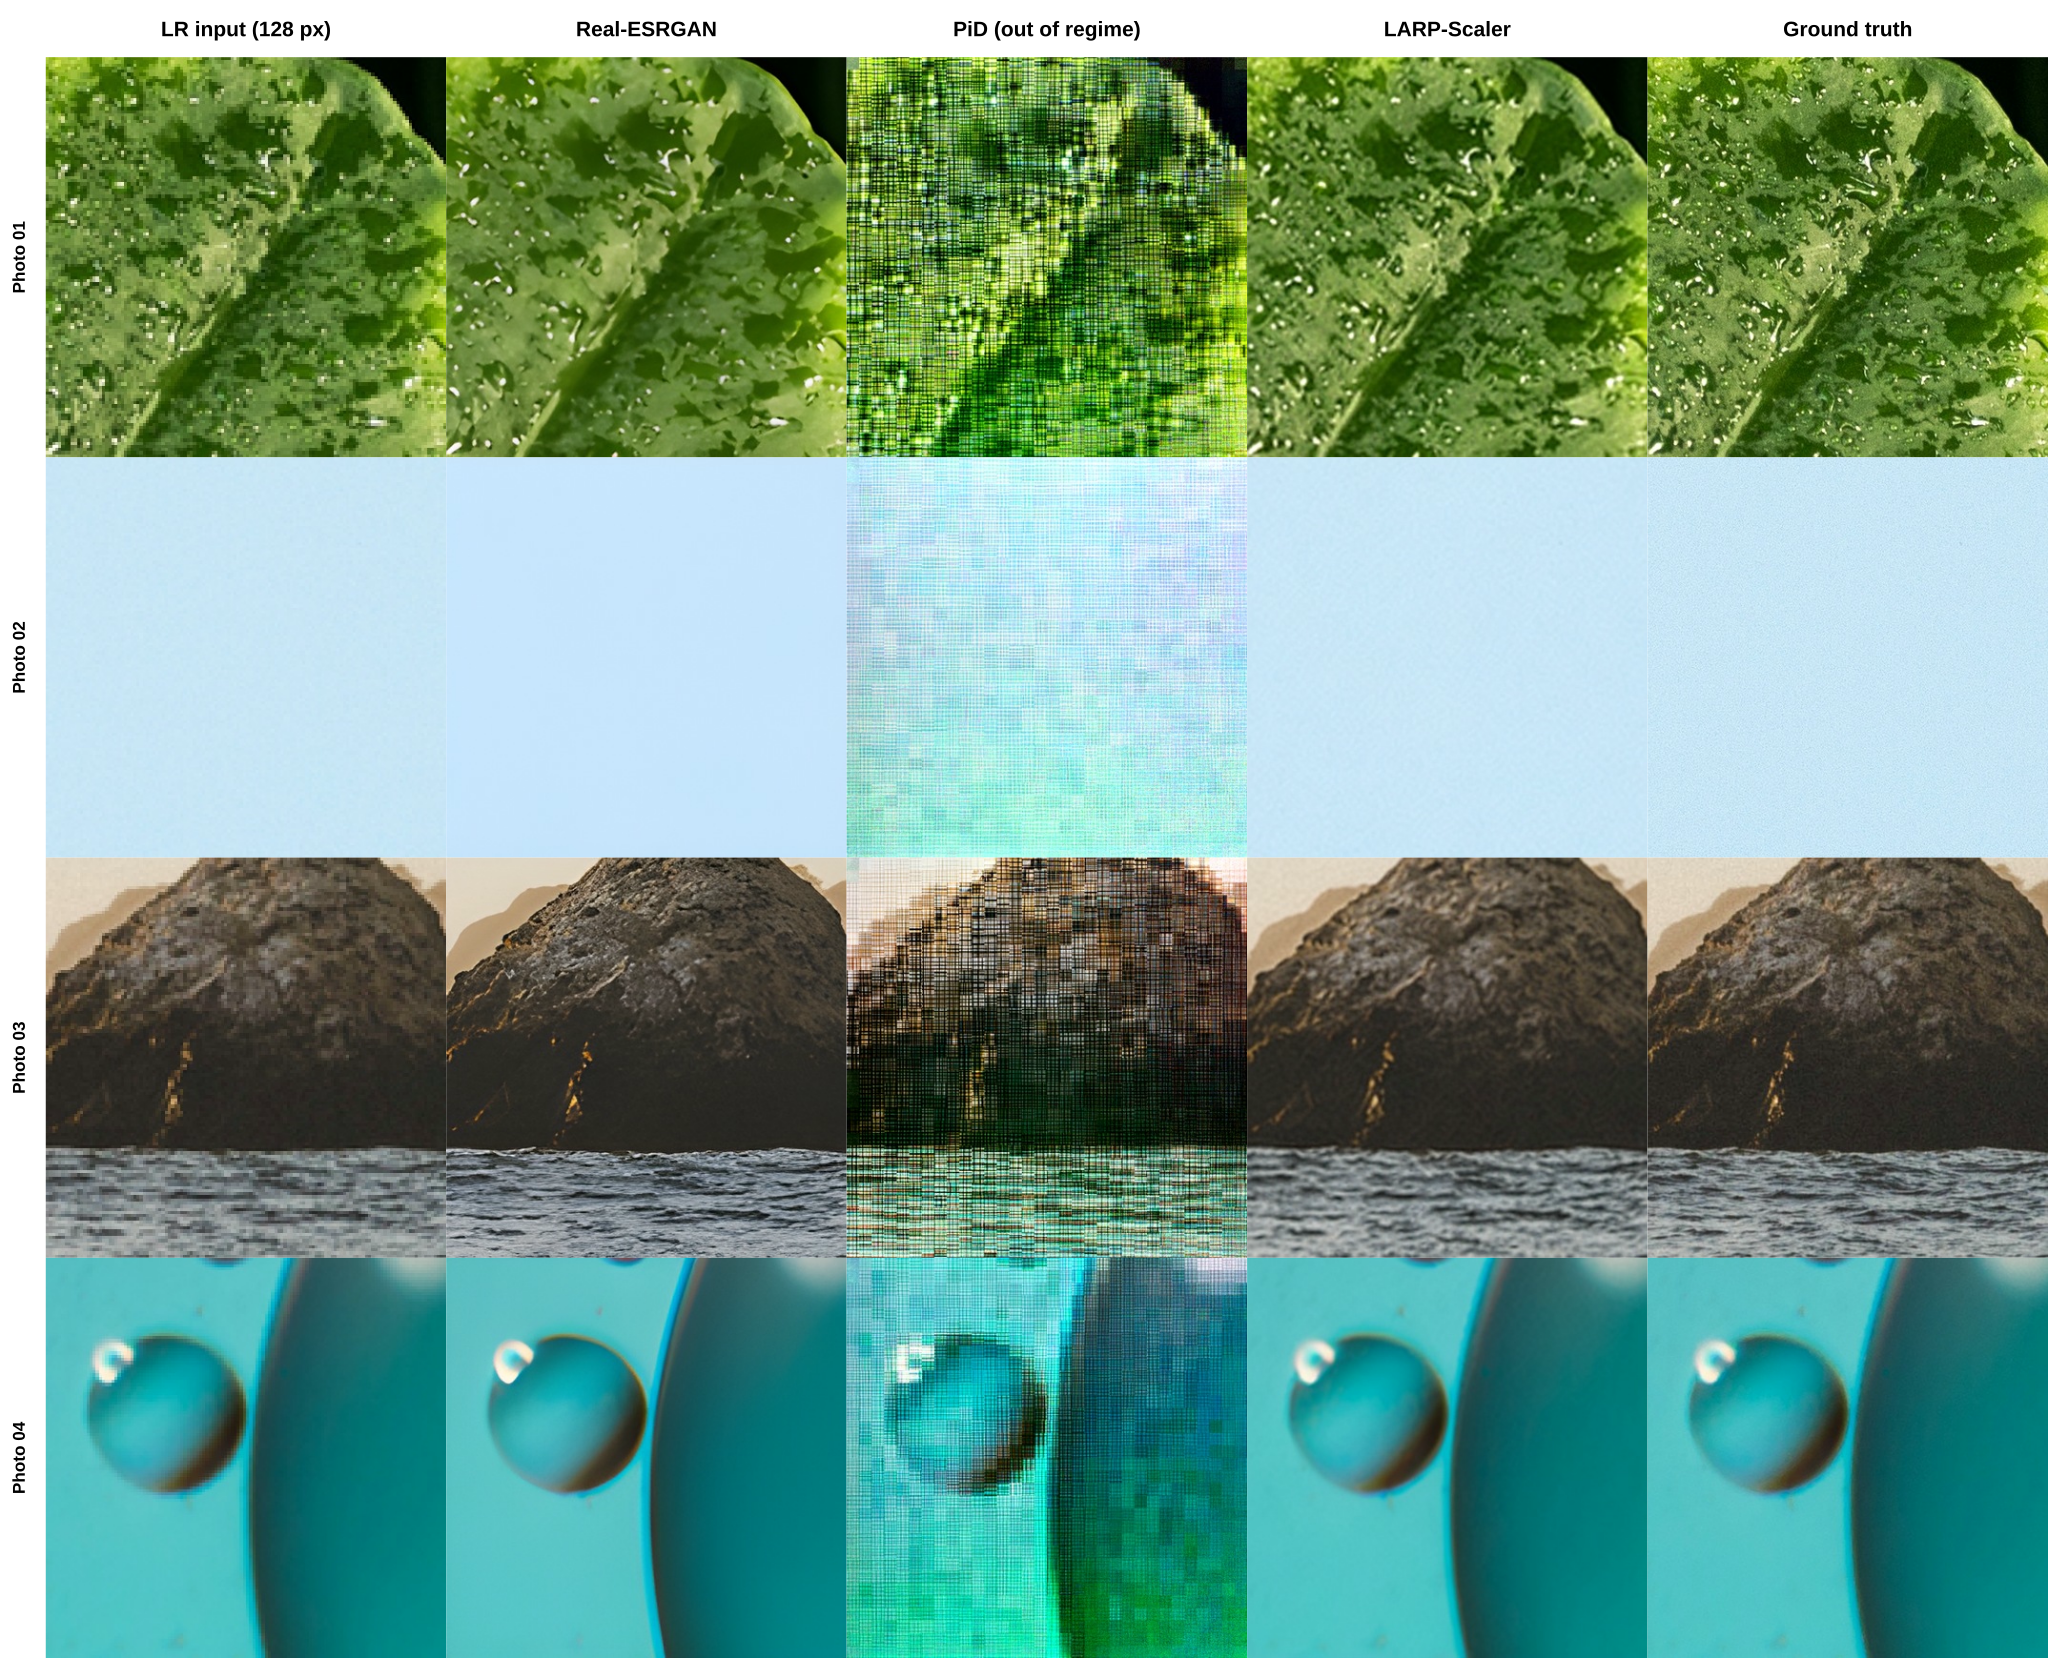
\includegraphics[width=0.95\textwidth]{figures/qualitative_comparison.jpg}
  \caption{\textbf{Native-2K qualitative comparison} at $4\times$
  ($512\!\to\!2048$). PiD uses its official
  \texttt{PiD\_res2k\_sr4x} four-step operating regime; all columns share the
  same LR inputs and targets. The four illustrative scenes cover fog and
  vertical edges, flower structure, water and rock detail, and smooth
  specular surfaces. Aggregate claims use all twelve images in
  \cref{tab:pid_native_quality}; these four rows are not a separate benchmark.
  The LR column is enlarged with nearest-neighbour sampling to expose its
  actual pixels.}
  \label{fig:qualitative}
\end{figure}
        \end{minipage}%

\end{strip}

% Keep the cross-method visual comparison near the end, on a dedicated
% full-width page rather than letting it disrupt the two-column discussion.
%\iffalse
%\clearpage
%\onecolumn
%\begin{center}
%\begin{minipage}{0.96\textwidth}
  %\centering
  %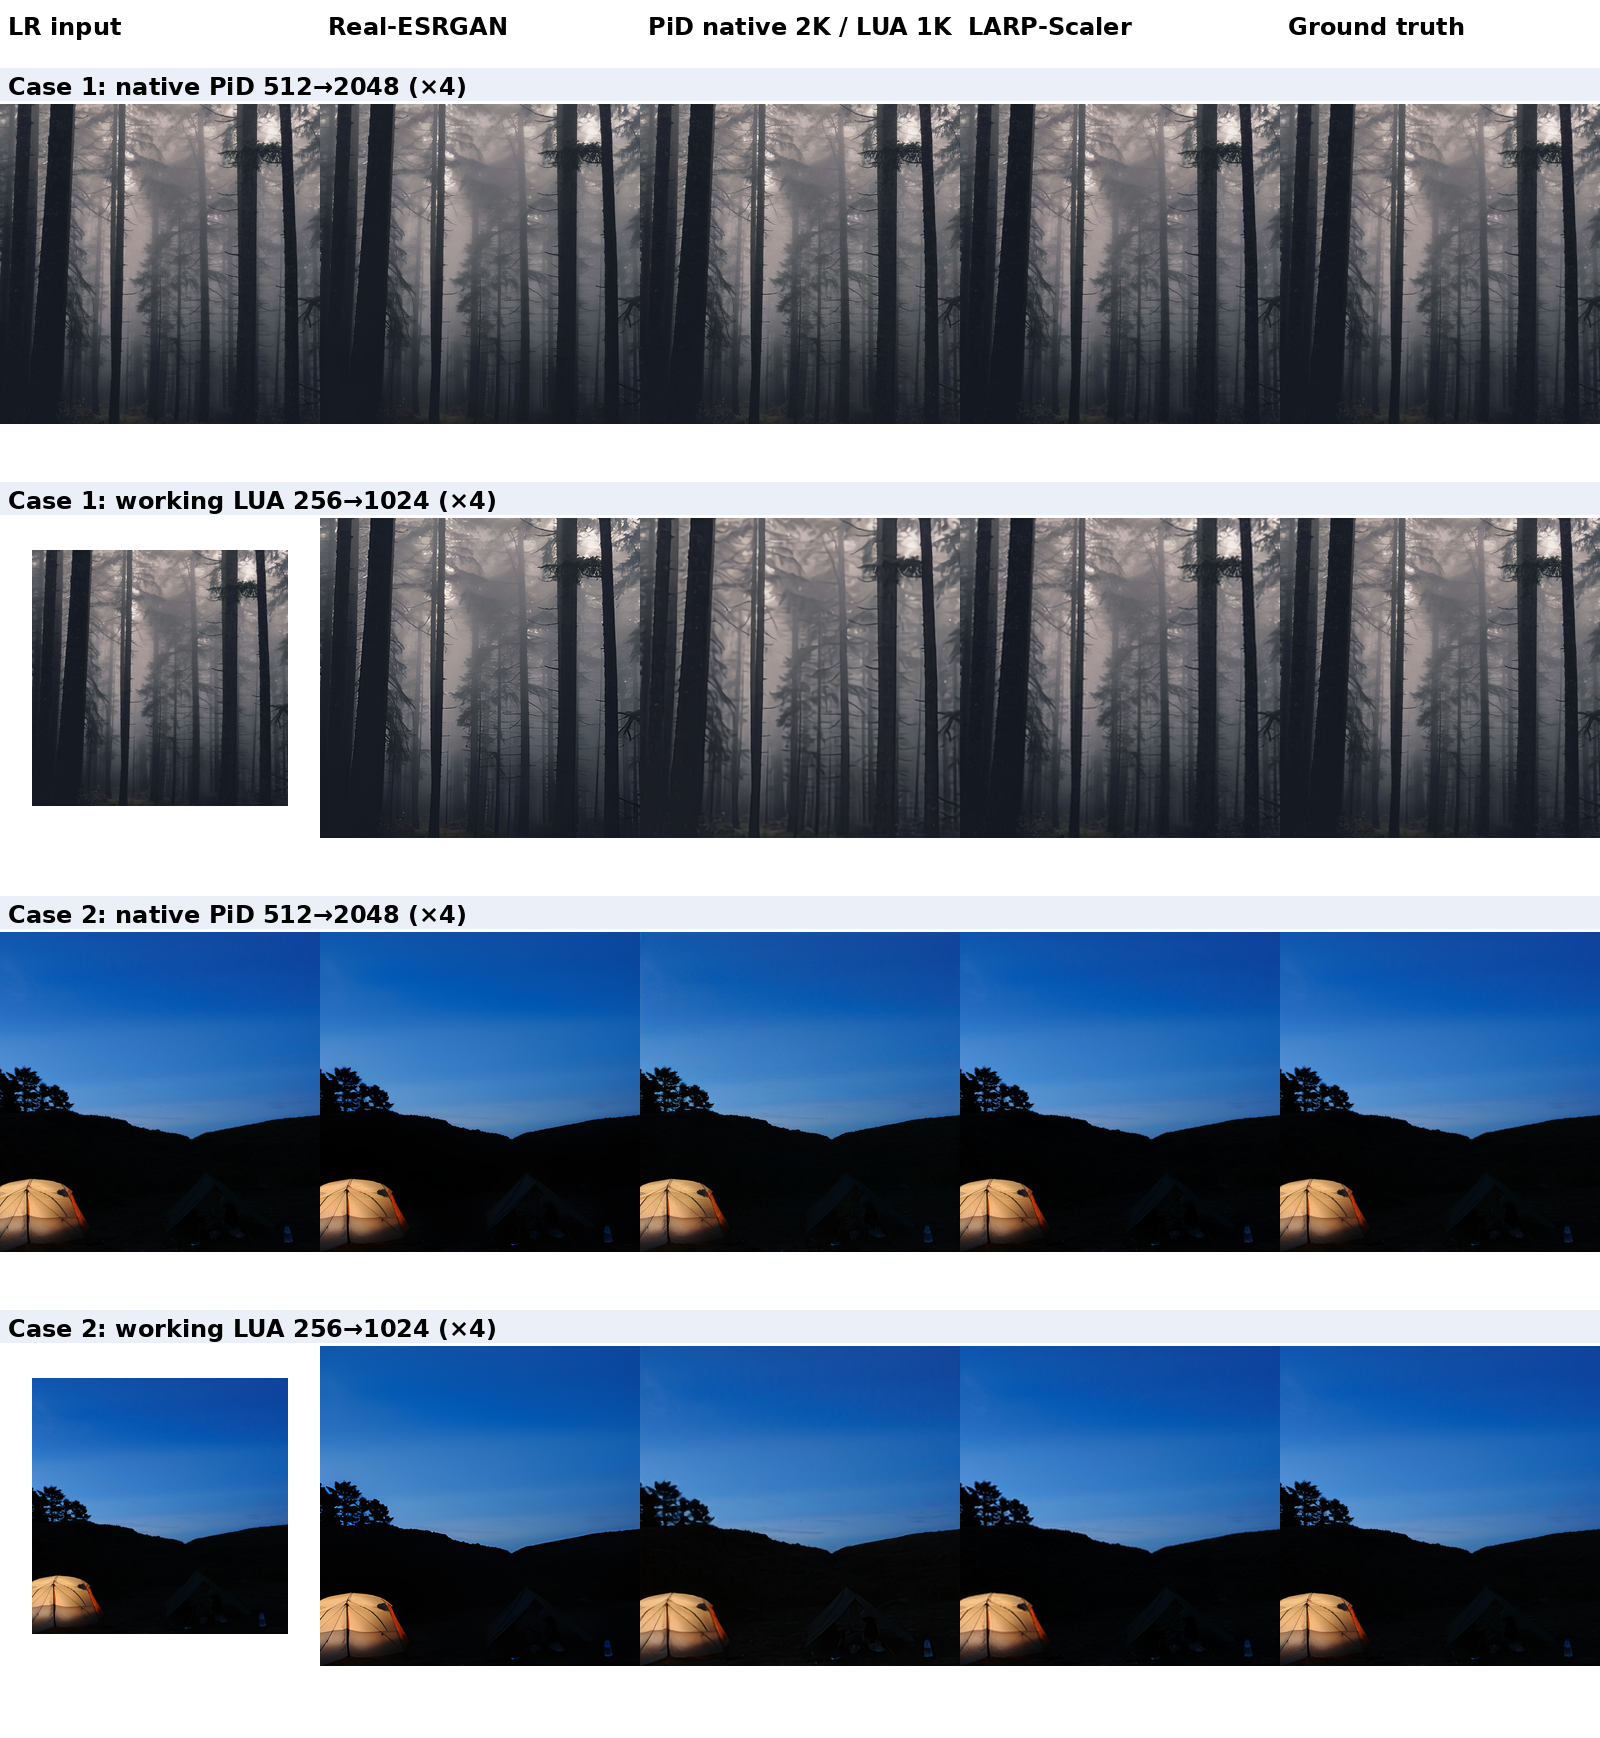
\includegraphics[width=\linewidth]{figures/larp_pid_lua_image_upscale_examples.png}
%\end{minipage}
%\end{center}
%\clearpage
%\twocolumn
%\fi
\section{Limitations}
\label{sec:limitations}

\paragraph{Small controlled sets.}
The main quality comparisons contain 12 photographs and 12 anime images. They
are controlled, reproducible reconstruction tests, but are not broad enough to
characterize rare domains, difficult degradations, faces, text, or pathological
compression. The separate 48-photo matrix improves scale coverage but does not
replace a broad public benchmark; bootstrap intervals on the 12-image sets are
wide.

\paragraph{Metric coverage.}
PSNR, SSIM, and MAE emphasize exact reconstruction and do not fully represent
perceptual quality. We additionally report LPIPS and DISTS
(\cref{tab:perceptual}), which show that a distortion-oriented lead does not
transfer uniformly to learned perceptual distances. No-reference IQA, FID, and
human preference remain unmeasured for the released checkpoint.

\paragraph{Protocol separation.}
Several additional measurements exist at other resolutions and on other image
sets. We report them separately in the appendix and do not combine them with
the shared tables. Cross-protocol deltas can suggest robustness but cannot be
added or treated as paired comparisons.

\paragraph{Hardware.}
Timing results use a single GPU family, the RTX 5090. Relative ordering may
change with memory bandwidth, kernel support, precision, CPU-side JPEG decode,
or different batch policies.

\paragraph{Compute availability.}
Access to computational resources was limited. Model development, the final
training stage, ablations, and evaluation used one four-GPU RTX 5090 machine.
This limited broad hyperparameter searches, multi-seed training, and
evaluation at substantially larger scale.

\paragraph{Training lineage and release artifacts.}
The recovered config and Trackio trace fully identify the final
direct-refinement stage, but the released model starts from a predecessor
SFT checkpoint at update 6,000. Consequently, 13.6 hours is final-stage wall
time rather than total end-to-end pretraining compute. The predecessor run is
identified in the machine-readable provenance, but its earlier initialization
contains restarted counters and is not summarized as a single total-compute
claim. The arXiv identifier remains pending.

\section{Conclusion}

We introduced \method, a SANA-based system that directly refines a target-sized
latent while conditioning on an independently encoded low-resolution image.
Cached text tensors and two-level tiling make the same checkpoint usable at
$2\times$, $4\times$, and $8\times$. On the two 12-image controlled sets,
\method leads the tested learned baselines in PSNR and MAE, while
protocol-matched interpolation retains the overall distortion advantage. The
separate 48-photo matrix confirms operation at all three scales and shows that
the PSNR gap to Lanczos narrows to 0.086 dB at $8\times$. Learned perceptual
metrics reverse part of the interpolation ranking: \method has lower LPIPS
than Lanczos and Bicubic on both controlled domains, while Bicubic narrowly
leads photo DISTS. The adapter-on ablation measures a
0.514 dB branch effect, but matched rather than mismatched guidance explains
only 0.079 dB under the same protocol. These results position \method as a
practical generative refinement system rather than a replacement for
conservative interpolation on paired distortion metrics. Broader public
benchmarks, real degradations, and human preference are the main remaining
evaluation priorities.

\bibliographystyle{unsrtnat}
\bibliography{references}

\clearpage
\appendix
\onecolumn
\section{Dataset Composition}

\label{app:dataset}

\begin{table}[H]
  \centering
  \caption{Final training metadata by source.}
  \label{tab:dataset_sources}
  \small
  \begin{tabular}{lr}
    \toprule
    Source & Records\\
    \midrule
    CommonCatalog & 100,046\\
    PD12M & 99,558\\
    4KLSDB & 43,977\\
    Unsplash & 24,849\\
    yande & 8,979\\
    konachan & 6,912\\
    danbooru & 2,982\\
    DIV8K & 1,000\\
    fine-t2i & 120\\
    \midrule
    Total & 288,423\\
    \bottomrule
  \end{tabular}
\end{table}

\begin{figure}[H]
  \centering
  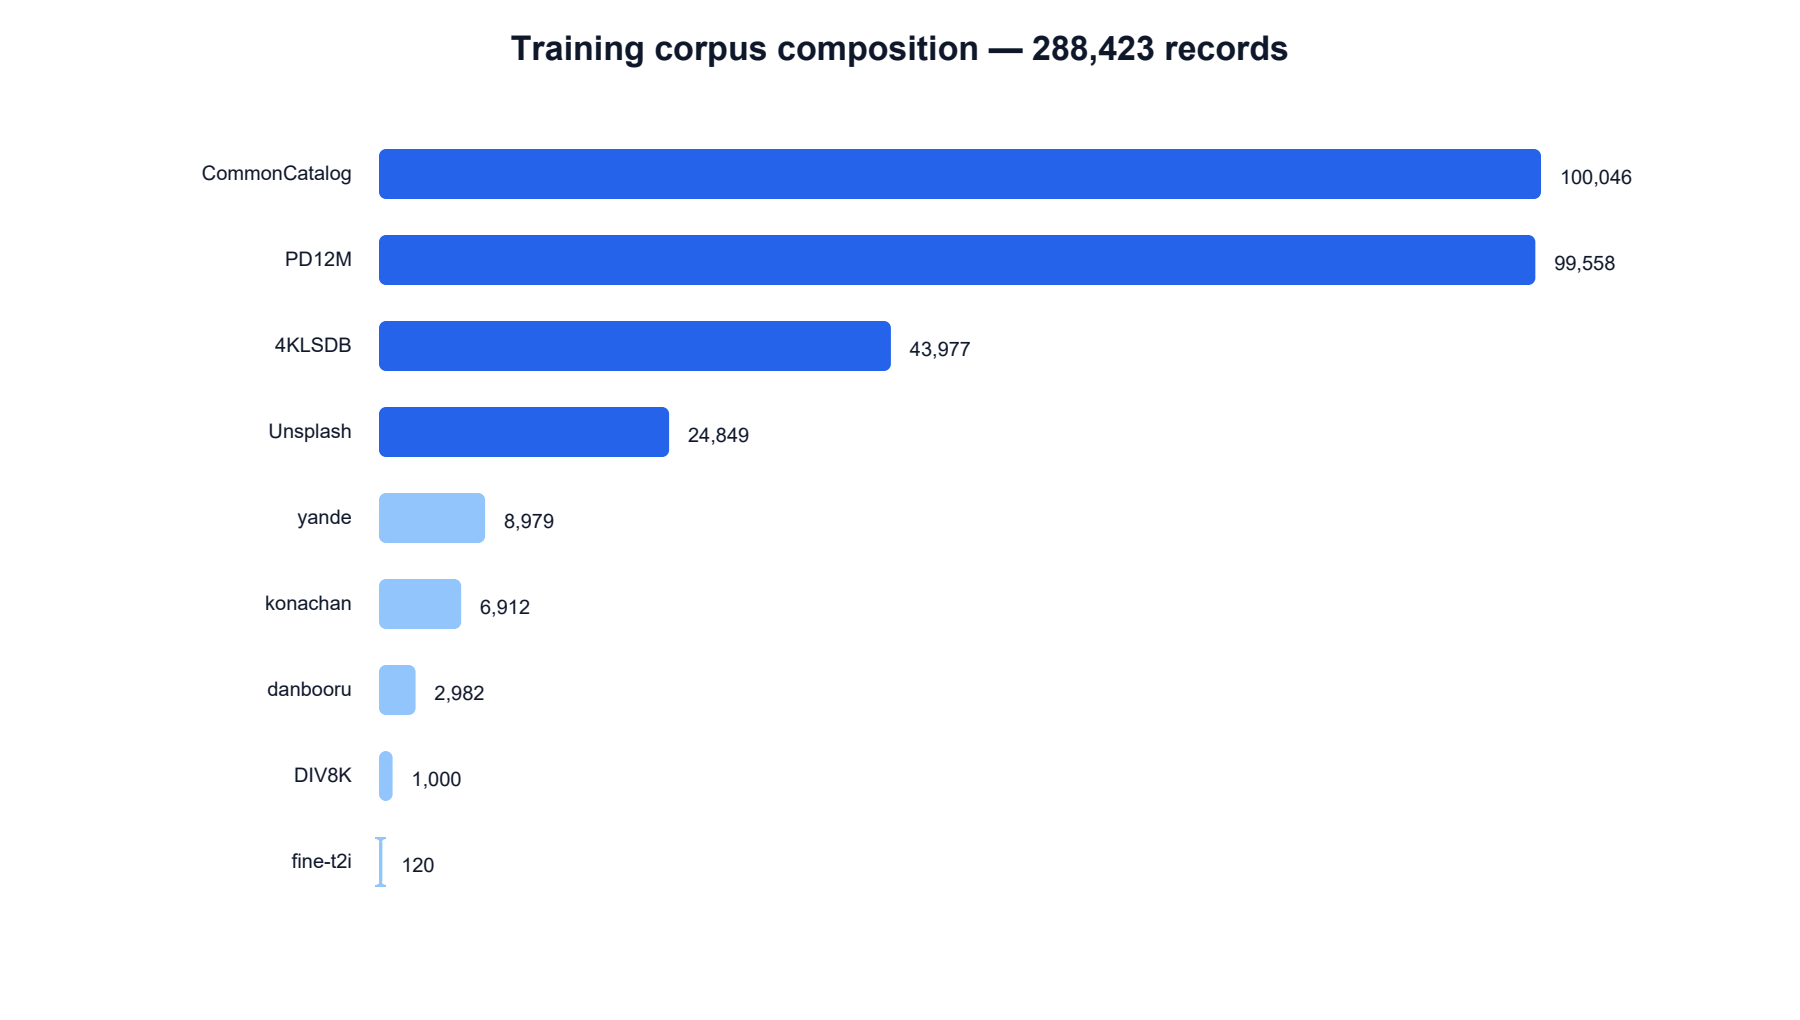
\includegraphics[width=\columnwidth]{figures/dataset_composition.png}
  \caption{Dataset source counts on a linear scale.}
  \label{fig:dataset_composition}
\end{figure}

\clearpage
\onecolumn
\section{Full Prompt--Adapter Matrix}
\label{app:ablation}

\begin{table}[H]
  \centering
  \caption{Prompt and adapter states, sorted by component rather than score.}
  \label{tab:full_ablation}
  \small
  \begin{tabular}{llccc}
    \toprule
    Prompt & Adapter & PSNR $\uparrow$ & SSIM $\uparrow$ & MAE $\downarrow$\\
    \midrule
    \multicolumn{5}{l}{\emph{Untrained SANA backbone (no direct-refinement stage)}}\\
    Empty & Off & 21.258000 & 0.696710 & 0.075979\\
    Detailed & Off & 21.255834 & 0.696634 & 0.076013\\
    Detailed + photo & Off & 21.262759 & 0.696799 & 0.075949\\
    \midrule
    \multicolumn{5}{l}{\emph{Released checkpoint}}\\
    Empty & Off & 31.285856 & 0.783891 & 0.024537\\
    Detailed & Off & 31.302412 & 0.783989 & 0.024495\\
    Detailed + photo & Off & 31.303990 & 0.783969 & 0.024491\\
    Empty & Matched guidance & 31.811783 & 0.787725 & 0.023156\\
    Detailed & Matched guidance & 31.817450 & 0.787747 & 0.023143\\
    Detailed + photo & Matched guidance & \textbf{31.817791} & 0.787734 & \textbf{0.023143}\\
    Detailed + photo & Mismatched guidance & 31.738986 & 0.787650 & 0.023208\\
    \bottomrule
  \end{tabular}
\end{table}

\section{Bootstrap Confidence Intervals}
\label{app:bootstrap}

We use percentile bootstrap intervals over images with 10,000 resamples and
seed 1234. Intervals are computed independently for each method, domain, scale,
and metric; no results from the 12-image and 48-image protocols are pooled.

\begin{table}[H]
  \centering
  \caption{Controlled $4\times$ reconstruction means and 95\% bootstrap
  confidence intervals. Each domain contains 12 images.}
  \label{tab:controlled_ci}
  \scriptsize
  \setlength{\tabcolsep}{4pt}
  \begin{tabular}{llccc}
    \toprule
    Domain & Method & PSNR [95\% CI] & SSIM [95\% CI] & MAE [95\% CI]\\
    \midrule
    \multirow{5}{*}{Photo}
      & Lanczos & 33.434 [29.756, 37.220] & 0.831 [0.774, 0.888] & 0.0191 [0.0123, 0.0270]\\
      & Bicubic & 33.236 [29.538, 37.017] & 0.825 [0.767, 0.883] & 0.0194 [0.0124, 0.0275]\\
      & \method & 31.817 [28.302, 35.267] & 0.788 [0.727, 0.851] & 0.0231 [0.0149, 0.0326]\\
      & Real-ESRGAN & 29.641 [26.485, 32.701] & 0.759 [0.688, 0.832] & 0.0285 [0.0184, 0.0397]\\
      & LUA & 19.554 [17.570, 21.441] & 0.407 [0.313, 0.502] & 0.0925 [0.0728, 0.1141]\\
    \midrule
    \multirow{5}{*}{Anime}
      & Lanczos & 28.794 [25.978, 31.982] & 0.865 [0.809, 0.912] & 0.0218 [0.0155, 0.0291]\\
      & Bicubic & 28.383 [25.739, 31.304] & 0.861 [0.806, 0.908] & 0.0219 [0.0157, 0.0291]\\
      & \method & 28.439 [25.931, 31.187] & 0.856 [0.802, 0.901] & 0.0238 [0.0177, 0.0308]\\
      & Real-ESRGAN & 26.785 [25.434, 28.047] & 0.869 [0.828, 0.901] & 0.0256 [0.0216, 0.0305]\\
      & LUA & 17.227 [16.441, 18.025] & 0.365 [0.329, 0.402] & 0.1097 [0.1004, 0.1190]\\
    \bottomrule
  \end{tabular}
\end{table}

\begin{table}[H]
  \centering
  \caption{Interpolation perceptual distances with 95\% bootstrap confidence
  intervals on the controlled $4\times$ sets. Intervals use 10,000 image-level
  resamples with seed 1234.}
  \label{tab:perceptual_interpolation_ci}
  \small
  \setlength{\tabcolsep}{5pt}
  \begin{tabular}{llcc}
    \toprule
    Domain & Method & LPIPS [95\% CI] & DISTS [95\% CI]\\
    \midrule
    \multirow{2}{*}{Photo}
      & Bicubic & 0.455 [0.351, 0.550] & 0.173 [0.141, 0.206]\\
      & Lanczos & 0.472 [0.363, 0.567] & 0.175 [0.144, 0.209]\\
    \midrule
    \multirow{2}{*}{Anime}
      & Bicubic & 0.296 [0.222, 0.370] & 0.125 [0.104, 0.141]\\
      & Lanczos & 0.293 [0.221, 0.365] & 0.127 [0.106, 0.142]\\
    \bottomrule
  \end{tabular}
\end{table}

\begin{table}[H]
  \centering
  \caption{Separate 48-photo multi-scale reconstruction means and 95\%
  bootstrap confidence intervals.}
  \label{tab:multiscale_ci}
  \scriptsize
  \setlength{\tabcolsep}{4pt}
  \begin{tabular}{llccc}
    \toprule
    Scale & Method & PSNR [95\% CI] & SSIM [95\% CI] & MAE [95\% CI]\\
    \midrule
    \multirow{3}{*}{$2\times$}
      & Lanczos & 36.647 [34.739, 38.495] & 0.912 [0.884, 0.936] & 0.0129 [0.0095, 0.0171]\\
      & Bicubic & 36.199 [34.314, 38.031] & 0.906 [0.876, 0.931] & 0.0134 [0.0099, 0.0177]\\
      & \method & 30.280 [28.637, 31.861] & 0.764 [0.716, 0.808] & 0.0245 [0.0194, 0.0306]\\
    \midrule
    \multirow{3}{*}{$4\times$}
      & Lanczos & 32.048 [30.322, 33.710] & 0.822 [0.777, 0.862] & 0.0197 [0.0151, 0.0253]\\
      & Bicubic & 31.841 [30.127, 33.491] & 0.817 [0.770, 0.858] & 0.0200 [0.0154, 0.0256]\\
      & \method & 30.789 [29.149, 32.363] & 0.787 [0.741, 0.829] & 0.0227 [0.0179, 0.0284]\\
    \midrule
    \multirow{3}{*}{$8\times$}
      & Lanczos & 29.202 [27.625, 30.714] & 0.735 [0.681, 0.785] & 0.0253 [0.0200, 0.0316]\\
      & Bicubic & 29.051 [27.486, 30.550] & 0.730 [0.676, 0.781] & 0.0256 [0.0202, 0.0318]\\
      & \method & 29.115 [27.566, 30.602] & 0.734 [0.681, 0.782] & 0.0259 [0.0206, 0.0320]\\
    \bottomrule
  \end{tabular}
\end{table}

\section{Implementation and Deterministic Settings}
\label{app:implementation}

The final direct-refinement stage uses training seed 6769, static loss scale
64, 1\% warm-up and cooldown, and a plateau controller with factor 0.8 and
patience 4. Three training workers use batch size 2 with 16 accumulation steps,
giving effective batch size 96; a fourth GPU produces frozen VAE and text
caches. The validation split uses seed 52. Validation runs every 100 updates
for eight batches with seed 1234. Stage boundaries restore BF16 model weights
but restart optimizer moments, scheduler history, RNG state, and data order.

All reported \method reconstruction and ablation runs use inference seed 1234.
The bootstrap uses an independent NumPy generator with seed 1234. Full
worker-level configuration and provenance remain machine-readable in
\path{paper/data/training_run.json}.


\section{Additional Cross-Protocol Measurements}
\label{app:extra}

The following results provide context but are not merged with the main shared
tables:
\begin{itemize}
  \item On 48 external photographs with 2048-pixel targets, the full trained
  system improves over native SANA by 8.976 dB at the best reported $4\times$
  setting.
  \item On a separate 32-photo adapter-control test, matched guidance exceeds
  mismatched guidance by 1.056 dB. This is larger than the 0.079 dB content
  effect on the 512-pixel ablation, demonstrating strong protocol dependence.
  \item Direct-refine checkpoint 4000 exceeds checkpoint 1000 by 0.047 dB on
  the reported 12-photo test.
\end{itemize}
These values should be read as robustness observations, not pooled estimates.

\section{Final-Stage Training Milestones}
\label{app:training}

\begin{table}[H]
  \centering
  \caption{Selected Trackio milestones for the released direct-refinement
  stage. The scalar training loss includes flow, reconstruction, and
  high-frequency components.}
  \label{tab:training_milestones}
  \small
  \begin{tabular}{rrr}
    \toprule
    Update & Train loss & Validation loss\\
    \midrule
    100  & 0.1640 & 0.1954\\
    500  & 0.1529 & 0.1672\\
    1,000 & 0.1526 & 0.1577\\
    1,500 & 0.1394 & 0.1534\\
    2,000 & 0.1452 & 0.1508\\
    2,500 & 0.1574 & 0.1494\\
    3,000 & 0.1420 & 0.1476\\
    3,500 & 0.1450 & 0.1466\\
    4,000 & 0.1288 & 0.1452\\
    \bottomrule
  \end{tabular}
\end{table}
\iffalse
\section{Reproducibility Checklist}
\label{app:checklist}

\begin{itemize}
  \item Public code and inference API: available.
  \item Public BF16 checkpoint: available.
  \item Machine-readable aggregate benchmark values: available in
  \texttt{paper/data/benchmarks.json}.
  \item Final-stage config, provenance, and Trackio milestones: available in
  \texttt{paper/data/training\_run.json}.
  \item Deterministic SVG/PDF figure generator: available.
  \item Exact quality and latency protocols: documented.
  \item Qualitative per-case outputs for four shared photographs, regenerated
  from the public checkpoint: available in \texttt{paper/qualitative/}.
  \item Independent re-run of the released package reproducing the reported
  per-image photo PSNR to within 0.003 dB: verified.
  \item Full per-image metric tables for all twelve photo and twelve anime
  images, including interpolation baselines: available in
  \texttt{paper/data/revision/controlled\_x4\_12\_per\_image.csv}.
  \item The 48-photo multi-scale per-image matrix and 95\% bootstrap intervals:
  available in \texttt{paper/data/revision/}.
  \item LPIPS and DISTS on both shared sets: available in
  \texttt{paper/data/perceptual\_metrics.json}.
  \item No-reference IQA, FID, and human preference: not measured.
  \item Public Gradio demo:
  \url{https://huggingface.co/spaces/Anonumous/LARP-Scaler}.
  \item arXiv page: pending.
\end{itemize}
\fi
\end{document}
